%
% Remi Beges PhD final report
%

% Page creation engine
\documentclass[11pt,a4paper]{book}
\usepackage[utf8x]{inputenc}
\usepackage[english]{babel}
\usepackage[T1]{fontenc}

% Main modules
\usepackage{url}      % URL
\usepackage[section]{placeins} % To ensure figures remain in their sections
\usepackage{siunitx}           % For proper unit formatting
\usepackage{graphicx} % Pictures
\usepackage{wrapfig}  % In-line Pictures
\usepackage{verbatim} % Code
\usepackage{mathtools,amssymb}
\usepackage[newfloat]{minted}   % Code
\usepackage[table,xcdraw]{xcolor} % For colors in tables
\usepackage{textgreek}% Greek language
\usepackage{booktabs} % Tables
\usepackage{colortbl} % For coloring rows, columns of table
\usepackage[toc,page]{appendix} % For managing appendix sections cleanly
\usepackage{algpseudocode} % For displaying pseudo-code
\usepackage{amsmath,empheq} % Math equations
\usepackage[nomain,acronym,xindy,toc]{glossaries}
\usepackage{makeidx}  % index support
\usepackage[ED=GEET-Elec, Ets=UT3]{tlsflyleaf} % Document cover
\usepackage{caption}     % float env with page breaks
\usepackage{hyperref}    % Links
\usepackage{bookmark}

% Package config
\newenvironment{code}{\captionsetup{type=listing,position=top}}{}
\DeclareSIUnit\sq{\ensuremath{\Box}}
\DeclareSIUnit\sample{S}
\DeclareSIUnit\div{div}
\bookmarksetup{open,numbered}

% Glossary
\loadglsentries{./src/glos}
\makeglossaries
\makeindex

% Front page
% Meta-data
%\title{Méthodologies d’analyse et de modélisation pour la prédiction de la robustesse fonctionnelle des circuits intégrés soumis à des agressions électriques transitoires}
\title{Analysis and modeling methods for predicting functional robustness of integrated circuits during fast transient events}
\author{Rémi Bèges}
\defencedate{2 juin 2017}
\lab{Laboratoire d'Analyse et d'Architecture des Systèmes (LAAS-CNRS - UPR 8001)}

% PhD mentors

\nboss{3}
\makesomeone{boss}{1}{Fabrice Caignet}{}{}
\makesomeone{boss}{2}{Patrice Besse}{}{}
\makesomeone{boss}{3}{Marise Bafleur}{}{}

% PhD Defence meta-data
%% Referee
\nreferee{2}
\makesomeone{referee}{1}{Mme. Geneviève Duchamp}{Professeur}{}
\makesomeone{referee}{2}{Mr. Pascal Nouet}{}{}
%% Judges
\njudge{8}
\makesomeone{judge}{1}{Geneviève Duchamp}{Professeur d'Université}{Membre du Jury}
\makesomeone{judge}{2}{Pascal Nouet}{Professeur d'Université}{Membre du Jury}
\makesomeone{judge}{3}{Alain Sauvage}{Docteur}{Membre du Jury}
\makesomeone{judge}{4}{Frederic Lafon}{Docteur}{Membre du Jury}
\makesomeone{judge}{5}{Fabrice Caignet}{Maitre de Conférence}{Membre du Jury}
\makesomeone{judge}{6}{Patrice Besse}{Docteur}{Membre du Jury}
\makesomeone{judge}{7}{Marise Bafleur}{Professeur d'Université}{Membre du Jury}
\makesomeone{judge}{8}{Patrick Austin}{Professeur d'Université}{Membre du Jury}

% Document
\begin{document}

\makeflyleaf

\tableofcontents

% Code highlighting styles
%\lstdefinestyle{veriloga-style}{
  language=Verilog,
  basicstyle=\footnotesize\ttfamily,
  commentstyle=\itshape\color{violet},
  identifierstyle=\color{blue},
  morekeywords={ border, buildmesh, cos, dx, dy, fespace, fill, func,
    int2d, label, mesh, on, pi, plot, problem, sin, real, x, y},
  % float,
  frame=single,
  numbers=left
}


\section{General introduction}

% Trends of the electronic field is size reduction
Electronic circuits become more miniaturized year after year.
There are many economical or practical reasons behind this trend.
Size reduction of integrated circuits lowers manufacturing cost per chip thanks to the increased volume.
Decreasing the weight of an embedded automotive system diminishes fuel and energy consumption.
Miniaturization also offers increased performance and capabilities.
More functions can be packed in the same volume.

% How is size reduced
For integrated circuits, this trend is accomplished by decreasing integrated technology size.
An integrated technology defines the dimensions and shapes of fundamental electronic bricks.
Those bricks consist in different types of transistors, resistors and capacitors.
The size of a technology is the smallest dimension for the smallest transistor gate, denoted \textlambda.
The value of \textlamda is essential and determines the size, power consumption, switching speed, performance and many other characteristics of the complete chip.
Until recently, Moore's law successfully predicted that technology dimensions will be reduced by a factor of two every 18 months.
As a side effect, miniaturization results in more fragile and less robust circuits.
%TODO detail more this
The maximum tolerated levels decrease with the technology size.

\begin{figure}[!h]
  \centering
  \includegraphics[width=0.3\textwidth]{src/1/figures/densification_integrated_functions.pdf}
  \caption{Increase of ECUs amount in a vehicle}
  \label{fig:ecus-increase}
\end{figure}

% Another trend in automotive - more electronic functions
Nowadays, new major features are developped in the automotive field.
The development of assisted or fully autonomous driving is seeing tremendous progress.
Autonomous vehicles take decisions and perform critical actions such as braking or steering the wheel.
Thoses features are implemented for safety purposes and put very high requirements on the operating safety of electronic modules.
Similarly, electric cars raise new challenges for safety, such as battery monitoring and control.
Those features require more computing power, more sensing capabilities and more data to exchange.
To support it, the amount of \gls{ecu}s and electronic modules is growing quickly in the automotive field.
Communication buses are shared by multiple systems, such as the CAN or LIN bus.
New standards and specifications are written to support higher bandwidths.
%TODO: Reference + complete
The CAN bus with Flexible Data rate (CAN-FD) is a good illustration.
Also means more sensitive to noise and disturbances.

% Another trend is reduced power consumptions
Another consequence of those trends is the rise of the vehicle's power consumption.
At the integrated circuit level, the main solution so far is to lower supply voltages.
With the smallest integrated technologies, it is common now to find supply voltages below 1V.
As a consequence, the noise margins become very small, making the circuits far more sensitive to electrical disturbances.

% Harsh environment in the automotive field
%TODO
On the other hand, the automotive field is a harsh environment for electronic devices.
Equipements are exposed to a wide range of mechanical, electrical and thermal stresses.
A running engine generates plenty of vibrations and mechanical stress.
Wear out electrical contacts, solder joints and connections.
It generates heat and thermal stress.
A vehicle can be exposed to large temperature variations during its lifetime.
Stress thermiques, vibrations, electriques, charges et decharges
definir ce qu'est un ESD EFT

% Architecture systemes automobiles
%TODO
A vehicle is constituted by a multitude of electronic modules, interconnected with cables.
This architecture is very challenging for robust against electrical disturbances
local ground reference potential differences, couplings between cables, cables and interference, etc.
SHowed that longer cables result in increased exposure to electrostatic discharges
Discuter article de renault pour les cables.

\begin{figure}[!h]
  \centering
  \includegraphics[width=0.3\textwidth]{src/1/figures/car_architecture.pdf}
  \caption{Architecture of electronic systems in a vehicle}
  \label{fig:car-architecture}
\end{figure}

% Fiabilite vis a vis des ESD
%TODO
So far, the current context is more electronics, complex systems, intrisically more fragile, and with more responsabilities.
It is obvious that all kinds of failures must preemptively be studied and predicted.
Definir hard failure, soft failure
Types de defaillance systeme, composant

% Recherche orientee jusqu'a la defaillance hardware
%TODO

% Comment predire ces defaillances fonctionnelles
%TODO
Recherche sur le fonctionnel a ses debuts
Beaucoup d'etudes au niveau systeme (mettre references de HDR fabrice)
Au niveau composant pas de methodes, peu d'etudes.

Recently, a new family of failures motivated new research work.
Those new failures are due to the multiple and recent trends for electronic devices, and in the automotive field.
In the last years, the amount of embedded electronic devices in vehicles has widely increased.
In parallel, the size reduction of semiconductor devices and technologies has continued, leading to reduced dimensions, reduced supply voltages and increased \gls{esd} sensitivity.
Finally, the development of smarter and autonomous vehicles are giving electronic devices more responsabilities in regard of our safety.
Now, they are commonly responsible for critical functions, such as airbag and braking control, and assisted or autonomous driving.
In this context, electronic devices are required to perform as expected with absolute reliability and without unpredictible behavior that could lead to castrophic consequences.
In particular, the functional robustness of this kind of devices must be guaranteed even in the event of an electrostatic discharge.

% Methodologies pour la conception - quel est le flot de design actuel
%TODO
Differents acteurs
Outils, simulateurs, etc
Comment on concoit un circuit
Actuellement, pas moyen de predire qu'un stress va generer un defaut fonctionnel
approche hierarchique, bottom up, top down

% Presentation des chapitres
%TODO
Chap 1 detaille ca, 2 detaille ceci, etc

% Chapter files listing
\chapter{Bibliography}

\section{Context}
\subsection{Electrostatic discharge}

%TODO
Electrostatic discharges are the result of the accumulation of potential.
Caused by tribocharging or electrostatic induction.
Sufficient potential is reached, a discharge happens.

% What are its key properties
Electrostatic discharges are very short events, usually in the range of a few hundred nanoseconds.
Currents in the range of tens of amperes are frequently observed and voltages of thousands of volts.
As a result, the overall discharge energy is small, but the power is extremely high.

% Impact
Harsh electrical disturbances are very harmful for electronic systems and integrated circuits.
Today, there is not a single electronic device in the field that is not protected against electrostatic discharges.
Due to the very short, fast, and random nature of \gls{esd} events, it remains very challenging to perfectly protect an electronic system against them.

% Especially for ESD
The automotive field has also the harshest requirements for \gls{esd}.
Several mechanisms generate static electricity accumulation when a vehicle is in motion \cite{generationESDautomotive}.
When electrostatic potentials become large enough, dielectric barrier breaks down and a discharge happens.
It propagates through the car's body, wiring and electronic equipments.
Electronic devices inside a car are therefore constantly exposed to electrostatic discharges.
They must be protected against it to avoid hardware failures or operating issues.

% Triboelectrification between tires and road surface
Triboelectrification can occur between the tires and and the road surface when a car is in motion \cite{generationESDautomotive}.
This process leads to the accumulation of electrostatic potential inside the car.
The capacitance formed between the vehicle and the ground effectively charges.
This effect is potentially countered by the vehicle leakage current to the ground.
If the triboelectric current is larger than the leakage, the capacitor charges anyway, until sufficiently a high potential potential is reached, at which point an electrostatic discharge is likely to happen.

% Triboelectrification between body and flow of air
%TODO: Find reference for this phenomenon
Troboelectrification can also occur for between the vehicle's body and the airflow generated by the motion.
More specifically, it is not the air itself but the particles carried in it that induce
Similarly, the friction between the car's body and the air flowing through it generates charge accumulation on the vehicle.

% Triboelectrification between a human body with clothing and the seat fabric
Triboelectrification may also happen between a human body with clothing and the seat fabric.
The probability of discharge is rather low \cite{generationESDautomotive} and may mostly happen when the human body leaves the vehicle, but it is still a possible source of \gls{esd}.

\subsection{Impact of ESD on electronic devices}

%TODO: Pictures
% Electronic devices are exposed to ESD, in factories first
As detailed in the introduction, electrostatic discharges constitute a large threat for electronic devices.
Failures can occur during manufacturing or normal operation.
The manipulation of parts by manufacturing machines involves repeated contact and separation.
Ultimately, triboelectrification and discharges happen and devices can get destroyed.
Several standards exist to guarantee that devices can survive this manufacturing step.

% HBM
The Human Body Model (HBM) reproduces the discharge of a human body into a device.
It is standardized in Method 3015.9 of MIL-STD-883 \cite{MIL-STD-883} and JEDEC JS-001-2014 \cite{jedec-001}.
The charged human body is modeled by a 100 pF capacitor and a discharge resistor of 1.5 k\textOmega{}.
Charging voltages reach a maximum of 8kV, although nowadays customers tend to ask for less than that.

% CDM
The Charged Device Model (CDM) is a field-induced ESD test.
The component under test is placed between two charging plates that generate an electric field.
At some point, a grounded pin is brought near any of the pins of the component, forcing the charges to evacuate suddenly.
This test is standardized in \cite{jedec-002}.

% MM
The Machine Model (MM) used to be another ESD testing specification that is now considered deprecated.
The JEDEC committee recommended discontinuing use of this standard \cite{discontinued-mm}, because it is the result of a misunderstanding of real-world events in manufacturing environments.
It does not help improving the reliability of devices against electrostatic discharges.

% HMM ?

%
Over the years, manufacturing processes and standards have improved, reducing the requirements of discharge levels to sustain.
In parallel, the factory environment has been studied extensively to identify actual levels devices are exposed to.
Machine Model deprecation is the perfect illustration of increased community knowledge and experience.
Those efforts aim to reduce the pressure on semiconductor manufacturers that are facing growing challenges to protect devices, because of the shrink of technologies and robustness.

% Electronic devices are exposed to ESD in the field
After manufacturing, failures can happen with the device in the field and exposed to its operating environment.
Manipulation by electrically-charged humans is a major source of danger for commercial products like cellphones and cameras.
The automotive environment is even harsher, with vehicles being a major source of electrostatic discharges.

% Main impact is hard-failure
The electrical destruction of a device is called a hard-failure.
A hard-failure corresponds to changes in the material structure or properties of a device to the point where it no longer fullfills at least part of its specification.
\gls{esd} induce those failures because of the extremely large current densities, high voltages, and power levels involved.
Different kinds of failure signatures can be observed.
Pictures of destroyed devices, obtained with an electronic microscope, are provided in Fig. \ref{fig:silicon-level-failures}.
%TODO: Comment

\begin{figure}[!h]
  \centering
  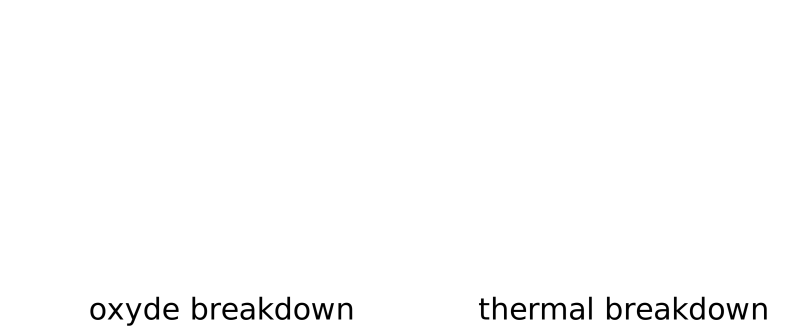
\includegraphics[width=\textwidth]{src/1/figures/esd_failures.pdf}
  \caption{Example of ESD induced failures at silicon-level (From \cite{esd-robust-product})}
  \label{fig:silicon-level-failures}
\end{figure}


% Oxide breakdown
%TODO: Etoffer avec these monnereau
A first kind of common failure for integrated devices is the oxide breakdown.
Oxide breakdown happens when an insulating material is exposed to a larger electric field than it can tolerate.
%TODO: Values
During an \gls{esd}, large voltage variations in a short amount of time result in very large electric fields superior to 1kV/m ?
For reference, thunder and lightning events have electrical fields in the same order of magnitude.
Oxide breakdown is usually discovered in the insulator constituting the gate of a \gls{mos} transistor.
As technologies shrink, so does transistor gate oxide thickness.
%TODO: thinner gate oxide can tolerate less electrical field ?
After the failure, the gate that is normally insulated from the rest of the device leaks significant amount of current.
The transistor can no longer operate and is considered destroyed.

% Thermal breakdown
Thermal breakdown is another kind of ESD induced failure.
It is the result of an elevation of temperature inside the silicon, above its melting point.
It is caused for long discharges that can induce significant and very localized device heating.
It results in a significant increase of leakage current or apparition of short-circuits.

% Metal melt
Finally, metal melting is the last kind of failures observed after a discharge.
Inside an integrated circuit, metal tracks are rather resistive because of their form factor.
Resistivity sits in the range of 10m\textOmega{}/$\Box$ to 100m\textOmega/$\Box$.
When large currents are flowing, metal tracks and vias dissipate power and heat up.
The elevation of temperature, if large enough, can melt the metal track and turn it into an open-circuit.

% Hard-failure is one thing, soft-fail another
Integrated circuits are studied and protected against hard-failure since a few decades.
Despite this experience of the \gls{esd} community, it remains challenging to perfectly protect an electronic system against hard-failures.
Nowadays, a new class of failures appears.
Instead of studying permanent failures, devices are studied for temporary failures affecting their functionality.
These are called soft-failures or functional failures.
\gls{esd} can cause them to happen, with diverse consequences.
In less severe situations, functionality of a chip is disturbed just for the duration of the ESD and recovers immediately without noticeable consequence.
The failure remains located inside the integrated circuit and does not impact the application above.
Sometimes, the discharge is harmful enough to cause a circuit to restart because the \gls{esd} disturbed some critical nets or parameters.
This is common when supply voltages go out of specification for instance.
Startups or power-on reset functions can interpret overvoltage or undervoltage caused by disturbances as the signal for a regular power-up sequence.
The device can also perform restarts to try a recovery because proper operations cannot be guaranteed, due to unexpected values on some nets.
Most microcontrollers for instance monitor supply voltages of digital gates.
If the voltage is too low, the noise margins of the gates cannot be guaranteed and proper operation either.
At this point, the microcontroller restarts to try to recover.
Restarts are slow processes compared to the operation of a chip.
For critical applications, this delay is highly unwanted because it impacts human safety.
The availability of the chip that triggers airbags in a car is vital for instance.
In a more severe scenario, the system gets completely frozen or stuck into an unwanted state because of the \gls{esd}.
The only way to recover normal operation requires a user-intervention.
User intervention can take the form of turning the key to shut down and restart the vehicle's engine.
Finally, hard-failure can be seen as the next step immediately after the most severe soft-failure.
The device is in a non-recoverable state and must be replaced.
Hard-failures are not considered for functional robustness analysis.

% What is the challenge
In this context, soft-failures represent a risk just as important as hardware failures.
To limit risks and costs inherents to upgrading a device after it was deployed in the field, these failures must be taken care of as early as possible.
Ideally, the robustness of an electronic product should be studied, characterized or simulated during its design phase.
The research conducted and presented in this document aims to develop new tools and techniques for studying and predicting functional failures.

% Protection of integrated circuits against hard-failure is done with ESD protections
To protect sensitive electronics against discharges, several options are available.
The most common solution, presented in the next section, is the \gls{esd} protection.

\subsection{ESD protection}

% Principle of operation
\gls{esd} protections deviate discharge current before it reaches sensitive circuitry.
By offering a low impedance path to ground, they clamp input voltages to avoid crossing the maximum accepted levels.
Fig. \ref{fig:esd-protection-strategy} gives a simple example of \gls{esd} protection strategy.
Current is routed into the ground before reaching the core circuitry.
Protections have very low on-resistance, usually in the order of a few ohms.
Even with a few amperes of current, voltage remains low.
\gls{esd} protections can absorb significant amounts of current for very short periods of time, but they are not designed to sustain DC currents.

\begin{figure}[!h]
  \centering
  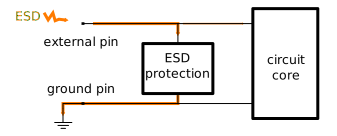
\includegraphics[width=0.8\textwidth]{src/1/figures/esd_protection_strategy.pdf}
  \caption{Classic ESD protection strategy}
  \label{fig:esd-protection-strategy}
\end{figure}

% Types of protection
Inside an electronic circuit, ESD protections are found in two different locations.
On-chip protections are integrated directly into silicon.
External protections are discrete devices connected to inputs or outputs of integrated circuits.
Historically, on-chip protections were designed for stresses generated during manufacturing.
They were not aimed to protect against system-level discharges, i.e. discharges happening in the field during the normal product life.
This task was fullfilled by external protections, such as transient voltage suppressors, diodes, capacitors, filters.
Over the years, design techniques and simulations tools have improved, and more robust integrated protections could be designed.
On the other hand, equipment manufacturer were always looking for means of reducing the \gls{bom} or the cost of electronic systems.
This led to a shift of responsabilities toward on-chip \gls{esd} protections for handling system-level stresses.
The shrink of integrated technologies makes this tasks even more challenging.
External protections are still very relevant, where an integration solution would occupy too much silicon area, or when very harsh requirements are demanded.

%TODO: These Monnereau : SEED Methodology - Collaboration entre protection interne et externe ?

\begin{figure}[!h]
  \centering
  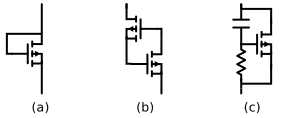
\includegraphics[width=0.8\textwidth]{src/1/figures/architecture_esd_protections.pdf}
  \caption{common ESD protections architectures - (a) Diode (b) Thyristor (c) RC-triggered MOS}
  \label{fig:architecture-esd-protection}
\end{figure}

% Implementation and common architectures
%TODO: These monnereau pr etoffer
ESD protections can be designed in various ways (see Fig. \ref{fig:architecture-esd-protection}).
Diodes are commonly found.
Thyristor architectures are frequently used too.
Thyristors have typical snapback characteristics as shown in Fig. \ref{fig:iv-curve-esd-protection}.
RC-triggered \gls{mos} are frequently found for protecting low-voltage \gls{io} of \gls{cmos} circuits.
Basically, it is a power transistor activated during the discharge by a resistor-capacitor network.
The capacitor is most of the time the parasitic gate capacitance to ground (TODO: check).
During a transient event, the capacitor acts as a short-circuit, rising the gate potential.
The \gls{mos} switches on and absorbs current, deviating it into the ground.

%TODO: Put leakage curve
\begin{figure}[!h]
  \centering
  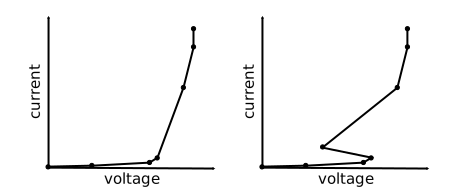
\includegraphics[width=0.7\textwidth]{src/1/figures/esd_protections_curves.pdf}
  \caption{I(V) curves of typical ESD protections with snapback and no-snapback}
  \label{fig:iv-curve-esd-protection}
\end{figure}

% Comment IV curve
A few key values are important for describing a protection.
V\textsubscript{t1} refers to the triggering voltage of the protection.
%TODO: snap only ?
I\textsubscript{t1} (snapback devices only ?) corresponds the current absorbed by the protection immediately after triggering.
V\textsubscript{t2} and I\textsubscript{t2} describe the coordinates where the protection is destroyed.
A sudden increase of the leakage current (Fig. \ref{fig:iv-curve-esd-protection}) is a good indicator of a damaged protection.

%TODO: Talk about protection strategies, centralized clamp vs distributed. RC-mos + boost rail to trigger all protections, etc.

% Requirements
To design an efficient \gls{esd} protection, several requirements are to be fullfilled.
In the absence of a discharge, protections must be transparent to the rest of the device.
The protection must trigger above the operating voltage of the circuitry.
For instance, if an input operates between 0V and 5V, and the protection switches on at 4V, it will trigger during normal operation and be immediately destroyed.
On the other hand, protections must clamp voltage (by absorbing current) before reaching the maximum voltage tolerated by the silicon technology.
They are designed to operate between those two boundaries which delimit the \gls{soa} (see Fig. \ref{fig:soa-esd-protection}).
For demanding applications, protections must trigger at a given voltage accurately, independently of manufacturing process, mismatches and temperature variation.
This reduces the \gls{soa} substantially and makes the design more challenging.

\begin{figure}[!h]
  \centering
  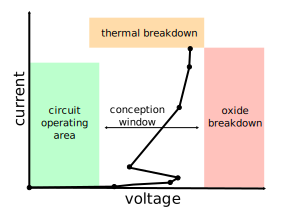
\includegraphics[width=0.3\textwidth]{src/1/figures/esd_protection_soa.pdf}
  \caption{Safe-Operating Area of an ESD protection}
  \label{fig:soa-esd-protection}
\end{figure}

% Tools
To design and validate protections, tools like Synopsys TCAD (Technology Computer Aided Design) \cite{tcad} are employed to simulate semiconductor physics.
Afterwards, an electrical model is constructed, to verify that the protection and the circuit cooperate as expected.
Simulation is ran in a \gls{spice} environment.
Modelling of \gls{esd} protections for \gls{spice} simulations is presented later in chapter \ref{esd-protection-modelling}.


\chapter{Development of investigation tools}
\label{chap:2}
\section{System-level modeling}

Simulations are a great tool to get a better understanding of the impact of \gls{esd}s on integrated circuits.
They allow introspection inside specific nets of the circuit, observe behavior that would be hard to observe in the field.
However, \gls{esd} simulations are not trivial, and like any simulation system, must be validated against measurement data before being used as an investigation tool.
Models for key devices must be derived, at each scale of the system.

In this chapter, the methodology for building models at the system level is detailed.
It mostly targets ESD generators and lab equipment.

\subsection{Transmission lines}

\gls{esd} events generally last a few hundred nanoseconds.

Any element that introduces a delay in the same order of magnitude (down to the nanosecond) can impact the waveforms.
Delays and propagation phenomena in general can obviously offset a waveform in time,
but also cause ringing oscillations with a period directly proportionnal to the delay.

Delays can be generated by cables and metal tracks, such as coaxial cables, twisted wires, wires over ground \gls{pcb} traces and so on.

Most cables and PCB traces, although of very different construction, usually behave as lossless transmission lines and can be modeled as such.

A transmission line is defined by two key parameters, a \gls{Zc} and a propagation delay.


For a purely lossless transmission line, the characteristic impedance is purely real.
In practice, truly lossless cables do not exist.
However, most coaxial cables exihibit very low losses below frequencies of a couple GHz, which is sufficient during ESD simulations to consider them lossless.

\subsubsection{Distributed model}

Physically, a transmission line is a distributed capacitance an inductance.
It can be modeled in a discrete manner, as a sum of unitary RLC elements.
The value for this unit element can be computed trivially from the characteristic impedance \gls{Zc}.

EQUATION RLC vs Zc

A single element generates a delay DT, much smaller than the delay of the cable.
To model the entire cable, many instances of this element are connected in series.
There is a tradoff to make between the delay of the unit element and the total amount of unit elements required to model the cable.

A small delay makes the cable model more accurate, however, more elements are required for the total cable, which results in longer simulation times.
On the other hand, a larger delay will limit the accuracy of the simulation by reducing the bandwidth of the model, which is not desirable either.

The main advantage for the distributed model is its ability to support lossy transmission lines (to check if this is true for a TL that has variable losses at low freqs).

The main disavantage is that it does not scales well with longer delays.
To keep the same bandwidth with a longer cable, the only solution is to increase the element count, resulting in longer simulation time.

\subsubsection{Behavioral model}

A behavioral model can describe efficiently and with great accuracy the behavior of most lossless transmission lines.

The electrical model is constituted of two voltage-controlled voltage sources and two resistors.
Compared to the classic RLC distributed model, the behavioral model has infinite bandwith, and constant complexity (compared to RLC where the amount of elements increases with the required bandwidth).

ELECTRICAL MODEL

EQUATIONS

The equations illustrate relations between incident and reflected waves, and voltage and current ratio.

\subsubsection{Conclusion on transmission line modeling}

To determine which model performs best, a few simulations are compared.
The test setup consist of a square pulse voltage source, with a risetime of 1 ps, a transmission line, and an unmatched termination at 25 ohms.

The RLC model with different settings is compared to the behavioral model.

cable 10ns, 50ns ?

- Config accurate
- Config fast
- Config lossy ?

Overall, the behavioral model outperforms the distributed model.
It is much more accurate (because not inherently limited in bandwith) and extremely fast to simulate.

The main reason for using the distributed model is to take losses into account, which is rather rare in practice.

\section{Modeling method application to a TLP generator}
\label{sec:tlp-modeling}

% Illustrate the method with a practical case
The methodology previously described in section \ref{sec:esd-modeling} is applied to the \gls{tlp} bench at NXP laboratory in Toulouse.
It is a good illustration on how to use the library of models for simulating a complete system.
Also, this particular testbench is widely used in NXP for characterizing and testing products.
The model described hereafter is used for instance to validate non-linear frequency model of passive devices.

% Describe the approach
To demonstrate its accuracy, the bench model is verified with an extensive simulation versus measurement comparison flow.
First, its behavior is measured under different loads and at different charging amplitudes.
The setup is identical for each simulation and measurement and is given Fig. \ref{fig:setup-cz-tlp-model}.

\begin{figure}[!h]
  \centering
  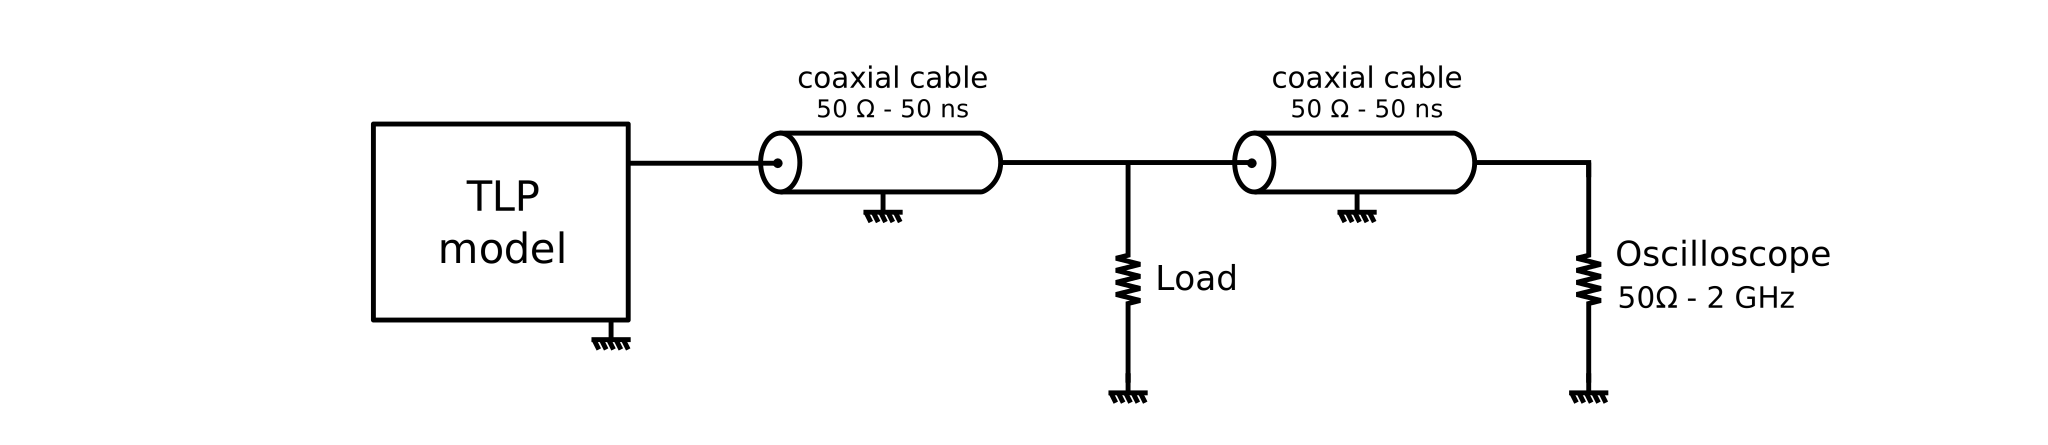
\includegraphics[width=\textwidth]{src/2/figures/tlp_characterization_setup.pdf}
  \caption{Characterization setup of the TLP}
  \label{fig:setup-cz-tlp-model}
\end{figure}

% Continue describing the approach
All the recorded time-domain waveforms serve as a reference for the modeling.
The list of test loads is constituted of resistors, capacitors and inductors of different values.
A first version of the testbench model is built, taking into account elements that physically exists.
It is tested with a first \gls{spice} simulation for a resistive load and charging voltage, and waveforms are compared against measurements.
If results correlate, the validation is continued with another load or another amplitude.
If results do not correlate, the model needs corrections.
Usually, some part of the curve will match the measurement, but others will not and call for improvements.
It can be convenient to try improving a single part of the waveform at a time.
Properties of time-domain reflectometry are helpful for locating where the model needs adjustments.
Indeed, with \gls{tdr}, a portion of the curve in time corresponds to a physical location inside the system.
If the fall time of the pulse is wrong for instance, then it can mean that some device that smooths the discharge is missing at the far end of the discharge cable.
It is also very convenient to observe pictures of the system taken during testing while building the model, because some small elements might easily be missed out or forgotten from the preliminary observation, yet they might impact waveforms a lot.
If some minor sections of the curves really cannot be matched using the system schematic as reference, then parasitic devices can be added.
All of these steps should quickly converge on an accurate ESD model.

\begin{figure}[!h]
  \centering
  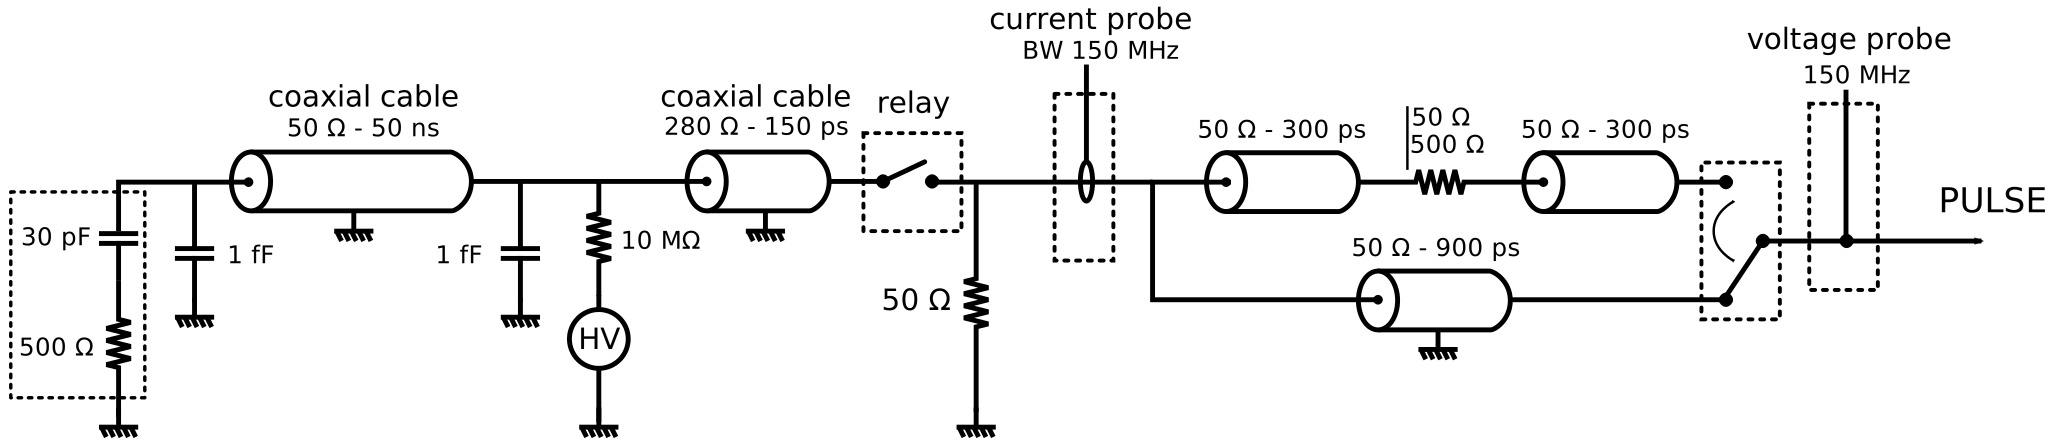
\includegraphics[width=\textwidth]{src/2/figures/complete_nxp_tlp_model.pdf}
  \caption{Complete model of NXP laboratory's TLP generator}
  \label{fig:complete-tlp-model}
\end{figure}

% Explain how the model, how it was constructed
The complete model is detailed in Fig. \ref{fig:complete-tlp-model}.
Similarly to all TLPs, the principle of operation is rather straightforward.
Initially, the relay is left open while the \SI{50}{\nano\second} coaxial cable on the left is being charged by the high voltage \gls{dc} supply.
The \SI{10}{\mega\ohm} resistor ensures that the cable charges slowly to avoid oscillations, and isolates the high voltage supply from the pulse.
The two \SI{1}{\femto\farad} capacitors placed at each end of the discharge cable help the simulator respect the initial condition for the charging voltage.
The cable is pre-charged to accelerate the simulation.
After the relay, a \SI{50}{\ohm} resistor can be found, intended as an attenuator.
Despite having a value of \SI{50}{\ohm} like the coaxial cables, this resistor creates an impedance mismatch.
It is the perfect illustration of a small element that is easily missed out but impacts waveforms a lot.
A current probe is connected immediately after the attenuator, and a voltage probe is connected at the output of the generator.
Position of the probes are important as well, to reproduce the timeshift between them.
The short transmission line represented by a \SI{150}{\pico\second} coaxial cable is a piece of bare wire.
It creates impedance mismatches because it has an estimated characteristic impedance of \SI{280}{\ohm}.
Finally, two discharge paths are possible inside the generator depending on the configuration of the switch on the output.
The direct path is at the bottom, where the pulse goes straight out from the generator.
The top path provides a series resistance that limits the discharge current.

% Detail a first comparison with 25 ohms
A first comparison between measurement and simulation is given in Fig. \ref{fig:comparison-tlp-load}.
With a \SI{25}{\ohm} resistor and a charging voltage of \SI{500}{\volt}, a current of \SI{4.5}{\ampere} (I\textsubscript{TLP}) and a voltage of \SI{125}{\milli\volt} (V\textsubscript{TLP}) are recorded.
The ratio of V\textsubscript{TLP}/I\textsubscript{TLP} between \SI{40}{\nano\second} to \SI{100}{\nano\second} is equal to \SI{25}{\ohm} as expected.
The small difference in the second step is due to a small mismatch between the defined charging voltage on the actual TLP bench and the value really applied onto the line.
It can be easily corrected in simulation by adding a small offset to the charging voltage.
Until \SI{220}{\nano\second}, both curves match closely.
After this time, some differences appear due to small modeling errors.
Because of the reflected waves, the errors accumulate and become significant, but only after the main part of the pulse.
Indeed, most ESD investigations focus on the part of the discharge below \SI{120}{\nano\second} which is the more relevant for the analysis because it actually represents voltage and current inside the device under test.

\begin{figure}[!h]
  \centering
  \includegraphics[width=\textwidth]{src/2/figures/tlp_comparison_R25_500V.png}
  \caption{Voltage and current waveforms comparison : \SI{500}{\volt} charging voltage on \SI{25}{\ohm}}
  \label{fig:comparison-tlp-load}
\end{figure}

% Second comparison with a short circuit
Same comparison is performed on a short circuit in Fig. \ref{fig:comparison-tlp-short}.
The goal is to test the extreme conditions where the model is going to be used.
As expected the voltage is null and the current is close to the maximum \SI{10}{\ampere} supplied by the TLP (\SI{500}{\volt} through \SI{50}{\ohm}).
At \SI{120}{\nano\second}, a large difference is observed between the two curves.
It is actually a measurement issue due to the oscilloscope clamping amplitude outside the observation window.
Because this is a limitation of the equipment, it is not modeled inside the simulation.

\begin{figure}[!h]
  \centering
  \includegraphics[width=\textwidth]{src/2/figures/tlp_comparison_short_500V.png}
  \caption{Voltage and current waveforms comparison : \SI{500}{\volt} charging voltage on a short circuit}
  \label{fig:comparison-tlp-short}
\end{figure}

% Third comparison on an open circuit
Finally, the process is repeated on an open circuit in Fig. \ref{fig:comparison-tlp-open}.
Observations are similar to the previous figures.
The voltage is recorded at \SI{220}{\volt}, corresponding to a bit less than half the TLP charging voltage.
For an ideal TLP, the value would be exactly \SI{250}{\volt}.
Due to the \SI{50}{\ohm} resistor between signal and ground inside this TLP bench, the voltage is slightly lower.
The current is close to \SI{0}{\ampere} because the load is an open circuit and does absorb current.
Between \SI{100}{\nano\second} and \SI{120}{\nano\second}, the same clamped measurement issue than previously is observed on the current waveform.

\begin{figure}[!h]
  \centering
  \includegraphics[width=\textwidth]{src/2/figures/tlp_comparison_open_500V.png}
  \caption{Voltage and current waveforms comparison : \SI{500}{\volt} charging voltage on open circuit}
  \label{fig:comparison-tlp-open}
\end{figure}

% Fourth load is capacitive
So far, only resistive loads were tested.
Capacitors are interesting to validate models with non real impedance.
The response of the generator on a \SI{1}{\nano\farad} capacitor is given in Fig. \ref{fig:comparison-tlp-capa}.
Between \SI{40}{\nano\second} and \SI{100}{\nano\second}, voltage and current are not stable, however measurement and simulation correlate well.
This is very interesting because it validates the behavior of the generator in dynamic regime, with large varying signals.
The near-linear voltage curve is due to the capacitor being charged at nearly constant current by the TLP.
The slope of this linear curve is directly related to the capacitor value.

\begin{figure}[!h]
  \centering
  \includegraphics[width=\textwidth]{src/2/figures/tlp_comparison_1nF_500V.png}
  \caption{Voltage and current waveforms comparison : \SI{500}{\volt} charging voltage on a \SI{1}{\nano\farad} capacitor}
  \label{fig:comparison-tlp-capa}
\end{figure}

% More validations in Annex
More simulation and validation curves are provided in Annex \ref{apx:tlp-validation-curves}, for different loads and amplitudes.
The goal of all those validations is to verify the model at both nominal and boundary conditions.
Overall, the model is good and fits very well the measurements, demonstrating the validity of the modeling method.

\input{src/2/sections/tlp-hmm.tex}
\subsection{On-chip near-field current measurement and postprocessing}
\label{sec:on-chip-near-field-process}

%TODO: Mathematical concept ?

\subsubsection{Time-domain integration method}

% Describe the algorithm
The time-domain method relies on the fact that the measured voltage is proportionnal to the derivative of the coupled current.
The algorithm begins with integrating the measured voltage, using a basic trapezoidal integration.
With the calibration sensor, it is possible to determinate experimentally the gain of the sensor.
%TODO: How is it done ?
Indeed, 1A of current does not generate 1V on the sensor, but a much lower value.
The correction factor with the current design was found to be $8.10^8$.
As a result of the integration, an offset is present a $t=0$.
So far, it is simply given the value of the calibration measurement at $t=0$.

%TODO: Give the result

% Limitations
The time-domain method is simple to compute.
However, it makes several assumptions on the sensor.
Mainly, it assumes that the gain of the sensor is constant for all frequencies.

\subsubsection{Frequency-domain reconstruction method}

The frequency domain tries to improve the post-processing by taking the sensor's response into account.
First, the sensor must be characterized, using a virtual network analyzer (Put glossary) (sure ?).
%TODO: Talk about complex measurement required
Then, the inverse of the sensor's characterization in the frequency domain is calculated.
%TODO: Is it really the inverse ?
%TODO: Give the formula

%TODO: Setup and Curve

In parallel, the FFT (glossary) of the measured waveform to post-process is computed.
For the algorithm to work, a complex FFT must be employed.
It computes for each frequency the amplitude and phase of the signal.

Afterwards, the FFT of the signal to process is multiplied by the inverse of the sensor's characterization.
Since both are complex numbers, real and imaginary parts must be multiplied separately, following complex-numbers algebra rules (source).

%TODO: Formula

Finally, the inverse FFT of the result is calculated to bring back the waveform into the time-domain.

% Talk about discrete
All waveforms, either measured experimentally or simulated, are constituted by a set of discrete points.
As such, discrete FFT and IFFT must be employed.

% Talk about repo
This post-processing method was implemented in python (ref).
It is freely distributed as open-source software (ref).

\subsubsection{Comparison of both methods}
This waveform can be compared with the original TLP stress used during calibration, and the curve reconstituted with the integration method.

\section{Conclusion}

% First section
In conclusion of this chapter, several tools have been presented for soft-failure analysis.
The system-level modeling method is very helpful to create accurate models, in order to simulate waveforms up to an integrated circuit.
It was a first required step before being able to study the apparition of functional failures inside integrated circuits, at the silicon level.

% Second section
The propagation and reflection mechanisms studied were used later on to create a custom pulse generator.
This new generator, called TLP-HMM, reproduces the waveform of the HMM specification and IEC 61000-4-2/ISO 10605 standards.
Combined together, they define the most widely employed pulse in the entire ESD field.
The TLP-HMM brings several advantages compared to a standard HMM generator.
Among other things, it offers advanced discharge reproducibility, a fully shielded propagation path and zero radiated emission.
The current design is a prototype that helped identify improvements to make in future iterations.
In particular, higher charging capability is required.

% Failure correlation
To test this generator against actual ESD guns, a set of 10 different ESD protections was stressed and destroyed with a TLP, a TLP-HMM and an HMM generator.
The comparison of failure levels between all of them led to discover a correlation law using the simplest possible equivalent circuit.
It relies on calculating the failure current, using the equivalent generator impedance, the ESD protection on-resistance and the charging voltage.
Then, calculating this failure current for one generator allows to guess the failing charging voltage of any other.
Charging voltages could be accurately guessed on the entire set of 10 protections.

% Near-field scan
Finally, two post-processing methods for a near-field on-chip probe were detailed.
The first method relies on an integration of the measured signal in the time domain.
The second method processes the signal in the frequency domain, by compensating it with the sensor characterization.
Accuracy of each method was grossly estimated.
Future work will involve a better assessment of the accuracy, and improvements to the processing script.


\chapter{Study of soft-failures at silicon-level}

\input{src/3/sections/section1_1.tex}
\section{Test vehicle}
\subsection{Test vehicle description}

% Why making a testchip
It is difficult to realize good measurements on an integrated circuit.
The chip is enclosed in a package, and without physical access it is impossible to measure electrical properties.
Even with physical access, placing micro-probes to contact metal connections can disturb sensitive parts of the device.
To overcome these issues, it is interesting to develop custom structures that perform the measurements directly on the chip and output the data using standard \gls{io}.
For that matter, a custom test vehicle has been designed and manufactured.

% What is in the testchip
The testchip reuses most blocks from the Everest product described previously in \ref{sec:study-real-product}.
%TODO: What is monitored
In addition, custom functions were integrated to allow the measurement and monitoring of internal parameters.
A communication system was setup to output measurement data using a few pins.

% Why monitoring a primary supply
The studied function is the primary supply of a complex automotive \gls{asic}.
This supply plays a critical role in the functionning of the entire product.
It is connected to the battery of the vehicle, and is the first block of the product to start.
It wakes up and powers all other functions inside the integrated circuit.

% Global architecture
The global architecture of the testchip (Fig. \ref{XX}) is comprised of a duplicated supply function.
The same supply block is instanciated twice on silicon.
One of them is the function under test, which is exposed to \gls{ESD} stresses and is monitored for failures.
The second one is responsible for powering the monitoring functions.
Both blocks are isolated from one another as much as possible.
The monitoring's supply is protected against disturbances to ensure good measurements.

\begin{figure}[h]
  \centering
  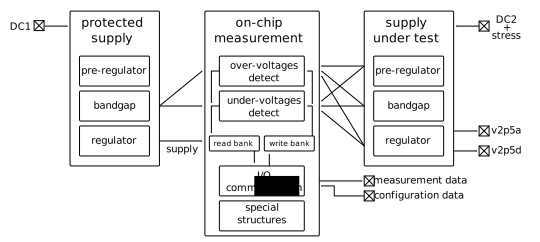
\includegraphics{src/3/figures/architecture_testchip.pdf}
  \caption{Global architecture of the test vehicle}
  \label{architecture_testchip}
\end{figure}

% What is in the monitoring system
The monitoring system is comprised of several functions.
Overvoltage and undervoltage detectors monitor voltage on nets in the supply under test.
The communication function performs a parallel to serial conversion, in order to read and write a large amount of bits using just a few pins.
Special structures for specific monitoring functions is also implemented.
Details about the monitored and monitoring functions are given in the next sub-sections.

\subsection{Monitored analog function}

The primary supply processes the battery supply in a chained fashion (see Fig. \ref{testchip_overview}).
A first block (pre-regulator) clamps the battery voltage (that can reach up to 40V) to 9V, a more acceptable voltage for the silicium technology.
This clamped voltaged is then used to power up a bandgap reference.
Once properly started, this bandgap generates a 1.23 V voltage reference, stable accross a wide range of temperature, process variation and mismatchs.
The bandgap also outputs a 10uA current reference, stable in the same conditions.

\begin{figure}[h]
  \centering
  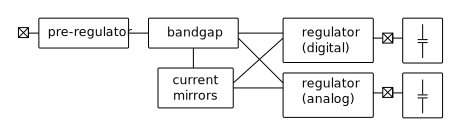
\includegraphics{src/4/figures/testchip_overview.pdf}
  \caption{Architecture of the studied functionnality}
  \label{testchip_overview}
\end{figure}

After the bandgap, a \gls{ldo} regulator relies on the voltage reference to generate a stable 2.5V supply voltage, able to deliver and sustain up to 20mA.
This first regulator is connected externally to a 100nF decoupling capacitor to absorb peak currents and achieve stability.
This supply is used to supply most analog (digital ?) functions inside the integrated circuit.

A second regulator performs the same task, but starts with a delay compared to the first one.
It also ouputs a 2.5V supply, that powers digital logic inside the circuit.

In case of failure, the primary supply can cause the entire product to shut down.
Indeed, this entire system requires soft-start behavior to avoid generating harmful voltage spikes to powered functions.
This functionnality enforces the system to start on a \br{long} period of time, in the order of a hundred microseconds.

When the system is stressed with an \gls{esd}, voltages and currents are fluctuating inside the block.
Under certain conditions, and especially important stress levels, the block will detects some nodes going in undervoltage or overvoltage.
This will cause the block to go into safe or protected mode, where it will restart because the functionnality cannot be assured properly.
The direct consequence is that the block will require again a hundred microseconds to be again in normal operation mode.

This failure can in a first time be observed in simulation.
An \gls{ESD} is superimposed on the DC battery voltage.
This is the most likely entry point for a stress, because the \gls{IC} exposes a pin to the external workd and is usally connected to the battery via a long cable
To detect is a block reset happened, the voltage on the first voltage regulator is observed.
Fig. X shows the stress waveform on the input.

STRESS WAVEFORM INPUT

Fig. X shows a simulation where a small glitch can be observed on the regulated output, but without clear reset or soft-failure signature.
In this case, the block and the rest of the product is most likely not affected by the ESD.

WAVEFORM OUTPUT NO RESET

Fig. X shows a simulation where a clear reset hapened.
The output voltage is maintained by a 100nF capacitor.
However, it clearly goes down \br{after} the \gls{esd} and rises slowly afterward, a sign that the block went into full reset and restard.

WAVEFORM OUTPUT RESET

By going inside the \gls{IC}...

bandgap, voltage ref, current ref, etc

DISCUSSION AROUND INCREASE OF FAILURE LENGTH after each stage of the chain

\subsection{Voltage monitoring}

% What are the OV/UV detectors made of
Overvoltage and undervoltage detectors are implemented with fast latched comparators.
The reference voltages for these comparators come from the protected supply.
The comparators monitor several key voltages inside the supply under test.
The output of these latched comparators form a register bank of 35 bits.

%TODO: Detail

\subsection{Communication system}

% What does the comm IO
The monitoring system also provides a bidirectionnal communication system.
It is designed to read with a single pin the values from the comparator register bank.
It also supports writing to a second register bank, that is used in the monitoring system for configuration.

%TODO: Detail

\subsection{On-chip near-field current sensors}

To be done
%TODO: Refer to PhD Alain
%TODO: Use document These/07

\subsection{Test boards}

% Why these board
For providing the external devices required by the testchip, and communicating with it, a master-slave architecture has been chosen.
The testchip is the slave, because it receives commands from the master for configuration and responds to reading requests.
One \gls{pcb} is designed for the master, and one for the slave.
The slave board contains the testchip and the required external devices.
The master board contains the microcontroller responsible for generating the frames for the testchip's monitoring system (section \ref{sec:comm-system-testchip}).
The master board connects to a computer for providing a user interface, reading, writing and storing the monitoring data.

% Overview of the setup
To protect the computer from \gls{esd} discharges, the two boards are isolated electrically.
Each board is powered with its own isolated battery, to avoid conducted stress propagating in the AC supply network.
The communication between the two is achieved with several optical fibers.
Optical communication is ideal because it completely isolates both boards electrically, and the fiber itself is completely immune to electrostatic discharges and more generally to electrical disturbances.
Each board packs its own set of optical to electrical converters, to make the conversion between the fiber and electrical signals.

\begin{figure}[!h]
  \centering
  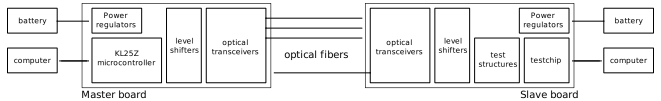
\includegraphics[width=\textwidth]{src/3/figures/boards_architecture.pdf}
  \caption{System architecture}
  \label{fig:system-board-architecture}
\end{figure}


%TODO: Picture?

\subsection{Test vehicle verification and testing after manufacturing}
\label{sec:test-vehicle-testing}

The testplan for the testchip is constituted of 7 steps, described in Fig. \ref{fig:verif-plan}.
The verification of the on-board voltage regulation is checked with a voltmeter, to ensure that a regulated 12V is well established.
The on-chip regulation is checked with a voltmeter and observed with an oscilloscope to validate the behavior.
All regulators from both boards and inside the testchip were found to operate as expected.

\begin{figure}[!h]
  \centering
  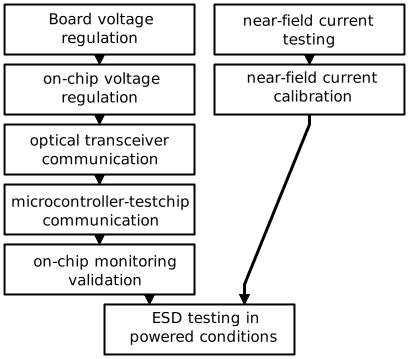
\includegraphics[width=0.7\textwidth]{src/3/figures/verification_plan.pdf}
  \caption{Test plan}
  \label{fig:verif-plan}
\end{figure}


\subsubsection{Optical communication}

% What is this step
The communication between the optical transceiver is verified.
Both the microcontroller and testchip were disconnected prior to injecting test frames on each transceiver.
Then, the output of the matching receiver was observed to ensure that the frame was properly transmitted.
Overall, minor issues were identified and corrected, and the boards were found fonctionnal.
This validates the physical layer of the communication.

\subsubsection{Master-slave communication}

The complete communication is then tested.
The microcontroller is used to send command frames such as reading requests on configuration data.
The testchip is supposed to respond each time with some specific data in return.
Unfortunately, very severe issues were found with this system.
After extensive debugging and testing, it was concluded that the communication could not work as-is and needed corrections.
As will be detailed later, the issue did not originally appear in the set of simulations ran during design to validate the entire test vehicle.
It required complex debugging steps such as parasitic devices extraction from layout to only partially reproduce the issue.

% How is the test done
The test is conducted by sending a reading frame multiple times.
By design, the integrated communication system expects a \textit{clk} signal with a frequency lower than 2MHz, and an \textit{en1} signal that must be high for a single rising clock edge.
With both these criteria met, the communication system should return the data on the \textit{data} pin.

% What is expected
By design, each frame incorporates a few mechanisms to ensure the returned data is correct.
Any \textit{data} frame must start with binary code 1010 and end with binary code 01.
The \textit{en1} signal set on the external input is propagated from one read cell to the next one.
The last cell of the chain is connected to the output pin \textit{en\_out}.
Confidence in the data is increased if the \textit{enable} signal (a pulse with a width of a single clock period) is observed on \textit{en\_out},

% What are the results
After attempting multiple readings with the same board, with different boards and different clock frequencies, the results are inconsistent.
Sometimes, the communication system returns an incomplete frame like in Fig. \ref{fig:read-only-partial-frame}.
In this case, the enable signal is not propagated correctly through the chain.
The \textit{en\_out} signal (not displayed here) stays low all the time.

\begin{figure}[!h]
  \centering
  \includegraphics[width=0.8\textwidth]{src/3/figures/read_only_partial_frame.pdf}
  \caption{Read-only partially returned frame (4ms/div, 5V/div) - clock frequency 1kHz}
  \label{fig:read-only-partial-frame}
\end{figure}

In other cases, the chain returns a complete but corrupted frame like in Fig. \ref{fig:read-only-full-frame}.
The enable is correctly propagated, and is visible on \textit{en\_out}, however the data start pattern is not correct (b'1011 instead of b'1010) and some intermediate digital values are not clearly defined.

\begin{figure}[!h]
  \centering
  \includegraphics[width=0.8\textwidth]{src/3/figures/read_only_corrupted_frame.pdf}
  \caption{Read-only corrupted frame (4ms/div, 5V/div) - clock frequency 1kHz}
  \label{fig:read-only-full-frame}
\end{figure}

%TODO: Detail more investigation
% Potential cause - clock freq
The clock frequency was initially suspected as a root cause for the problem.
Previous measurements were taken for a slow 1kHz clock frequency, which is far slower than the upper limit 2MHz.
Increasing the clock frequency at 10kHz, 100kHz and 1MHz did not improve the situation.

% Potential cause - delays
The impact of parasitic delays causing the communication system to malfunction was also suspected.
Multiple simulations of the entire read chain were run by placing large delays in multiple locations.
No failure could be highlighted using this method.

% Potential cause - parasitic RC
Afterwards, an RC parasitics were extracted from the layout.
Once again, the read chain performed correctly.

% Potential cause - susbstrate coupling
Susbtrate couplings were also suspected.
Some reading issues could be reproduced, but this type of coupling is highly unlikely to happen for clock frequencies of 1kHz.

%TODO: Detail simulations + what was done to reproduce problem

\subsubsection{Future work}

% Multiple bonding diagrams
A second revision of the testchip is planned.
Since the investigation on the communication system is unconclusive, it was decided to remove it.
Instead, detectors will be directly connected to pads, and most test or validation structure will be removed.
To overcome the problem of low available pin count, it is possible to put on silicon more pads than the amount of external pins.
Then, two different bonding diagrams will be made to connect each part of the available pads, to be able to use all detectors.



\chapter{Modeling of IC for operating ESD simulations}

\section{Bottom-up block failure modeling}
\label{sec:bottom-up-modeling}
%TODO: Introduction

\subsection{Block failure characterization and modeling method}
\label{sec:block-failure-cz}

% What is bottom up
In a bottom-up approach, the study focuses first on the small-scale components of a system.
They are characterized individually, and a model is derived for each component.
Afterwards, these models are assembled together to match the full system architecture.
The main idea of a bottom-up approach is that a system is the sum of its parts.
Ultimately, we study if the robustness of a system can be assimilated as the sum of the robustness of its parts.
%TODO: Detail more

% Applicability to IC design
This approach fits well with the \gls{asic} design flow in general.
At some point in the design flow, the architecture of the integrated circuit is decided.
Then, each top-level function is split recursively into unit functions to be designed, to simplify the problem.
This part is rather a divide-and-conquer method, where a complex problem is split up into multiple simpler tasks.

Then, the design phase starts. It is a bottom-up method.
Transistors are assembled together to perform (usually one) unit function into what is called a \gls{block}.
Those blocks are then assembled together to build the more complex and interesting functionnalities.

% Why bottom up
The main perk of this characterization method is the inherent modularity.
The objective is to study each block independently of the others.
This way, the model built for each block is reusable.
A characterized block can be reused multiple times without having to do the characterization again each time.

% How is it done, core concept
The method described in this section starts by characterizing each block in a particular setup.
This setup provides appropriate biasing to the block, in order to set it in normal operating conditions.
This setup is also in charge of injecting the characterization signal on the tested input, and monitoring of the output under test.
Fig. \ref{block_function_cz} gives an example of such a characterization setup for a supply input.

%TODO: Improve figure (text sizes)
%TODO: Remove range comparator
\begin{figure}[!htbp]
  \centering
  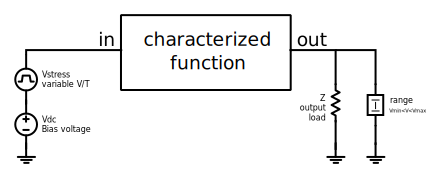
\includegraphics{src/4/figures/characterization_setup.pdf}
  \caption{Block characterization setup (supply input)}
  \label{block_function_cz}
\end{figure}

% What are the characterization signal
The characterization signal is a square waveform, applied on the tested input.
A set of simulations is ran with this setup.
Each simulation runs with a different pair of values for the \textbf{amplitude} and \textbf{duration} of the square signal.
Table \ref{parameterized-simulations} illustrates this simulation process.
Such testing method is called Wunsch and Bell in the litterature (REFERENCE).

\begin{table}[!htbp]
\centering
\begin{tabular}{@{}lllll@{}}
\toprule
    & 1ns   & 10ns  & 100ns & 1\textmugreek{}s   \\ \midrule
5V  & sim11 & sim21 & sim31 & sim41 \\
10V & sim12 & sim22 & sim32 & sim42 \\
15V & sim13 & sim23 & sim33 & sim43 \\ \bottomrule
\end{tabular}
\caption{Parameterized simulation planning for the characterization}
\label{parameterized-simulations}
\end{table}

In the time domain, this set of simulations is illustrated in Fig. \ref{set_input_signals}.

%TODO: Fix sim 12 sim12
\begin{figure}[!htbp]
  \centering
  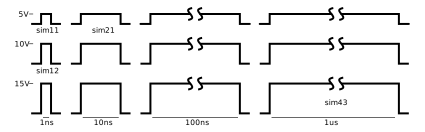
\includegraphics{src/4/figures/time_domain_cz_curves.pdf}
  \caption{Variations on (amplitude, duration) of the input characterization signal}
  \label{set_input_signals}
\end{figure}

% What is the direct result of the characterization, how to obtain it
For each simulation, the waveform of the output under test is recorded.
The waveform is compared against a threshold.
This threshold can also be seen as failure criteria of the studied function.
%TODO: Donner un example : If we consider the pre-reg block, the failure criteria will be ...

This treshold is set prior to the simulation.
There is no general rule for setting it.
The \gls{dc} specification of the output can be used directly, if it exists, or a sound value in regard of the design, or an arbitrary level.

If the waveform goes above (maximum threshold) or below (minimum threshold), the simulation is marked as \textit{fail}.
For each simulation, the duration during which the failure criteria was violated is also recorded.
Once all simulations are complete, it is known which ones contain a \textit{fail}.

The results are summarized into table \ref{simulation-results}.

\begin{table}[!htbp]
\centering
\begin{tabular}{@{}lllll@{}}
\toprule
    & 1ns                          & 10ns                         & 100ns                        & 1\textmugreek{}s             \\ \midrule
5V  & {\color[HTML]{32CB00} sim11} & {\color[HTML]{32CB00} sim21} & {\color[HTML]{32CB00} sim31} & {\color[HTML]{FE0000} sim41} \\
10V & {\color[HTML]{32CB00} sim12} & {\color[HTML]{FE0000} sim22} & {\color[HTML]{FE0000} sim32} & {\color[HTML]{FE0000} sim42} \\
15V & {\color[HTML]{FE0000} sim13} & {\color[HTML]{FE0000} sim23} & {\color[HTML]{FE0000} sim33} & {\color[HTML]{FE0000} sim43} \\ \bottomrule
\end{tabular}
\caption{Example of results on a set of simulations (simulations in red contain a fail)}
\label{simulation-results}
\end{table}

% A first visualization of the characterization
A curve can be build from this table, to make visualization easier.
It gives a visual representation of the functionnal robustness of the block.
Following table \ref{simulation-results}, the x axis is the duration of the input stress.
The y axis is the amplitude of the input signal during the stress.
This amplitude is the voltage or current seen by the characterized input pin.
It is the sum of the stress amplitude and an eventual biasing level.
Finally, each point (x,y) of the curve represents the \textbf{minimal} amplitude (y) for the given pulse width (x) at which failures occur.

Fig. \ref{wb_cz_curve_example} gives an example of such a characterization curve.

%TODO: REVOIR COULEURS
\begin{figure}[!htbp]
  \centering
  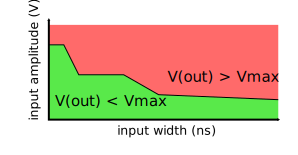
\includegraphics{src/4/figures/example_curve.pdf}
  \caption{Principle of Wunsch and Bell curve for powered-on block testing}
  \label{wb_cz_curve_example}
\end{figure}

% How to improve the displayed information
The duration during which an output is in fail was recorded for each simulation, as stated earlier.
% WHY IS THIS IMPORTANT
It is possible to improve table \ref{simulation-results} by replacing the \textit{fail} by the duration of the fail.
This is illustrated in table \ref{simulation-results-bis}.

\begin{table}[!htbp]
\centering
\begin{tabular}{@{}lcccc@{}}
\toprule
    & \multicolumn{1}{l}{1ns}      & \multicolumn{1}{l}{10ns}     & \multicolumn{1}{l}{100ns}    & \multicolumn{1}{l}{1us}     \\ \midrule
5V  & {\color[HTML]{32CB00} }      & {\color[HTML]{32CB00} }      & {\color[HTML]{32CB00} }      & {\color[HTML]{F56B00} 2us}  \\
10V & {\color[HTML]{32CB00} }      & {\color[HTML]{00D2CB} 125ns} & {\color[HTML]{F8A102} 540ns} & {\color[HTML]{FE0000} 30us} \\
15V & {\color[HTML]{00D2CB} 110ns} & {\color[HTML]{FFCB2F} 150ns} & {\color[HTML]{FE0000} 30us}  & {\color[HTML]{FE0000} 30us} \\ \bottomrule
\end{tabular}
\caption{A more informative representation of all simulation results to account for duration of output failure}
\label{simulation-results-bis}
\end{table}

% How to improve the curve from the improved table
This improvement can also be transfered to the curve representation.
A gradient can be used rather than a simple failure curve.
For each point of the curve, the gradient will have a value representing the duration of the failure on \textbf{\textit{V(out)}}.
The figure \ref{wb_cz_curve_example_v2} provides an example of this improved representation.
In this figure, the warmer the gradient, the longer the output is disturbed.

\begin{figure}[!htbp]
  \centering
  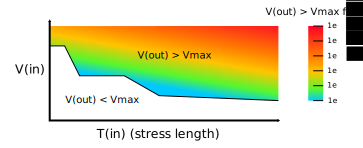
\includegraphics{src/4/figures/example_curve_v2.pdf}
  \caption{Improved curve for Wunsch and Bell powered-on characterization}
  \label{wb_cz_curve_example_v2}
\end{figure}

The gradient can also be discretized into a few aeras for better readability as shown in figure \ref{wb_cz_curve_example_v2_discrete}.
This representation looses some information compared to the gradient one, but is easier to generate and read.
This is the representation we have adopted further in this study, to express the functionnal robustness of a single block.

\begin{figure}[!htbp]
  \centering
  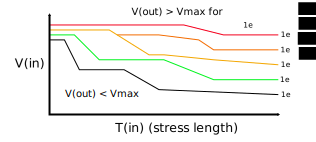
\includegraphics{src/4/figures/example_curve_v2_discrete.pdf}
  \caption{Improved discrete curve for Wunsch and Bell powered-on characterization}
  \label{wb_cz_curve_example_v2_discrete}
\end{figure}

\subsection{Block models chaining}
\label{sec:block-chaining}

% Explain the chaining mechanism
The characterization process detailed previously (in \ref{sec:block-failure-cz}) is repeated on each block constituting a high-level function.
Once done, the bottom-up study now focuses on a higher level in the design hierarchy.
As a remainder, the original goal of this method is to see if the robustness of a high-level function is the sum of its parts' robustness.

Thus, individual models are connected together, by following exactly how blocks are connected in the design.
To illustrate this idea, fig. \ref{example_toplevel_function} represents an example of a high-level function, constituted of three blocks at the second level of hierarchy.
It is assumed that each of these blocks has been characterized.

% WHICH NET IS TOP MONITORED ?

\begin{figure}[!htbp]
  \centering
  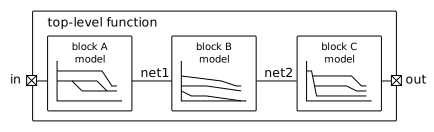
\includegraphics{src/4/figures/example_top_level_function.pdf}
  \caption{Example of a top-level function with 3 characterized blocks}
  \label{example_toplevel_function}
\end{figure}

% Remind the final goal
Now, we want to obtain the robustness of the entire function, against a given stress, using the block models.
The stress is injected on the global pin \textbf{\textit{in}}.

% What is the input stress ? What is the top-level function evaluated against ?
In this example, we will consider the stress is generated by a \gls{tlp} generator, and is thus rectangular.
For this example, the stress is chosen to have a duration of 100 ns, and an amplitude of 10V.
Section \ref{sec:wb-for-arbitrary-wvfs} describes methods for applying the block models to arbitrary input waveforms.

% How is used the characterization of the output of A on the input of B ?
%TODO: Detail a lot more. This is key. Speak about modeling of the output, and simplification to square pulse.
%TODO: Make a figure to show how is the disturbance on the output of A is modeled
The stress is injected on the global \textbf{\textit{in}} pin.
This pin is also the input pin of the first block.
Thus, the properties of the \gls{tlp} pulse can directly be applied to the model of block A.
Fig. \ref{example_complete_curve} shows an example curve for model A, and the location of the TLP pulse characteristics on this curve.


\begin{figure}[!htbp]
  \centering
  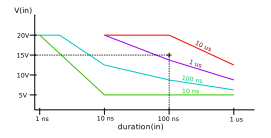
\includegraphics{src/4/figures/example_complete_curve.pdf}
  \caption{Model A curve and determination of impact of the TLP pulse - values in color represent the duration of failure on the output}
  \label{example_complete_curve}
\end{figure}

% Interpretate stress to deduce net1
Like stated earlier, the pulse has a duration of 100ns and an amplitude of 15V. By reporting this point on curve \ref{example_complete_curve},
it is visible that this will cause the output of block A to violate its failure criteria between 1 \textmugreek{}s and 10 \textmugreek{}s.
We consider, for the sake of this example, the failure criteria of block A to be net1 > 5V.
With a 100ns long 15V pulse on the input of A, the characterization states that the output of block A will go above 5V for at least 1us.
This is the best case value for net1.

% Use net1 as input of next block
\textit{net1} is the output of block A, but it is also the input of block B.
Thus, best case (amplitude, duration) values for net1 can be used as input for block B's model.
Fig. \ref{example_complete_curve_B} shows an example curve for model B, and the location of the \textit{net1} disturbance on this curve.
This shows that \textit{net2}, the output of block B and the input of block C, will go below B's failure level for at least 10 \textmugreek{}s.

\begin{figure}[!htbp]
  \centering
  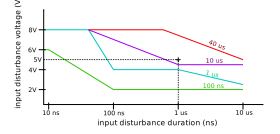
\includegraphics{src/4/figures/example_complete_curve_B.pdf}
  \caption{Model B curve and determination of impact of the TLP pulse}
  \label{example_complete_curve_B}
\end{figure}

% Repeatable process
As shown, this process can be repeated in theory with as many blocks as required by the original design, until the final pin is reached.
The is possible because the output of a block is used as the input of the next one.

%TODO: Algorithm organigram

% How to select pins to characterize

% Show how it can help to speedup and simplify the computation of the entire function robustness

\subsection{Application to the test vehicle}

The method described in both previous sections (\ref{sec:block-failure-cz} and \ref{sec:block-chaining}) is tested in simulation on real blocks.
More precisely, it will be tested against the regulation function of the testchip.

% Which pins are selected for characterization
This function is composed of three blocks, a pre-regulator, a bandgap and a regulator.
For each one, an input and output pin are selected.
The input/outputs that play a key role on the regulation function were selected on the regulation function.
Details of the selected pins is given in Table \ref{selected-pins-for-cz}.

%TODO: To simplify
\begin{table}[]
\centering
\begin{tabularx}{\linewidth}@{}|c|c|c|c|c|c|c|@{}}
\toprule
{ \textbf{IC block}} & { \textbf{input pin}}                 & \multicolumn{1}{l|}{{ }} & { }                                & \multicolumn{1}{l|}{{ }}               & { \textbf{output pin}}            & { }                          \\ \midrule
{ }                  & { \textbf{specification}}             & { \textbf{DC value (V)}} & { \textbf{stress amplitude range}} & { \textbf{stress width range}}         & { \textbf{specification}}         & { \textbf{Failure criteria}} \\ \midrule
{ pre-regulator}     & { external supply battery connection} & { 12V}                   & { -1V to -10V with 1V step}        & { 1ns to 1000ns with 30 pts log scale} & { 9V clamped voltage}             & { vclamp9 \textless 0V}      \\ \midrule
{ bandgap}           & { 9V clamped voltage}                 & { 9V}                    & { -1V to -15V with 1V step}        & { 1ns to 1000ns with 30 pts log scale} & { bandgap voltage 2.5V reference} & { vref2p5 \textless 1.25V}   \\ \midrule
{ regulator}         & { bandgap 2.5V reference}             & { 2.5V}                  & { -0.5 to -10V with 0.5V step}     & { 1ns to 1000ns with 30 pts log scale} & { regulated 2.5V 20mA capability} & { v2p5 \textless 2.1 V}      \\ \bottomrule
\end{tabularx}
\caption{Selected pins for characterization and characterization limits}
\label{selected-pins-for-cz}
\end{table}

% Talk about the characterization limits
The characterization is done using negative voltages.
The goal is to exploit the weakness of the testchip against negative pulses discovered and highlighted in section \ref{sec:testchip_study}.
Basically, it was observed for sufficiently high negative voltage a short pulse can cause a full restart of the system.
The time taken by this restart, observed on the regulator output, is several order of magnitudes longer than the original pulse injected on the pre-regulator input.

% failure criteria chosen
The failure criteria for the pre-regulator is a voltage lower than 0V on the output.
It corresponds to a situation worse than the unpowered state, where all nets are at 0V.
The failure criteria for the bandgap is a voltage lower than 1.25V on the 2.5V reference output.
Finally, the failure criteria for the regulator, which is also the failure criteria for the complete function, is a voltage lower than 2.1V on the 2.5V regulated output.
This criteria corresponds to a voltage below which digital cells using this supply will fail to function properly.

% Which load value for characterization
The test setup described in section \ref{sec:block-failure-cz} requires a characterization load to simulate the impact of neighbor blocks.
In a first time, a very simplistic model is employed for this load.
An arbitrary load value of 1M\textgreek{Omega}\ is initially chosen, just to perform a preliminary test.
The impact of this load on the characterization will be evaluated later on in the analysis.

% Simulation process
For each block, the characterization testbench is setup and a set of simulations is ran.
This set is calculated with the characterization range given in Table \ref{selected-pins-for-cz}.
This type of parameterized simulations can be efficiently distributed on multiple machines.
This way, the complete characterization of a block does not take longer than the time taken by a single simulation.
Once all simulations are run, the results are analysed and plotted using the method detailed in the previous sections.

% Talk about the output
These characterization curves are given in Figs. \ref{pre_regu_wb}, \ref{bandgap_wb} and \ref{regu_wb}.
The characterization of the pre-regulator (fig. \ref{pre_regu_wb}) is plotted using the stress amplitude only on the X axis.
The stress amplitude is the pulse voltage set in the pulse generator SPICE model.
On the other hand, the bandgap and regulator curves are using instead the voltage probed on the input net during the stress.


% TODO: Why curve 1 has different x-axis
The reason for using the set voltage directly, and not

\begin{figure}[!htbp]
  \centering
  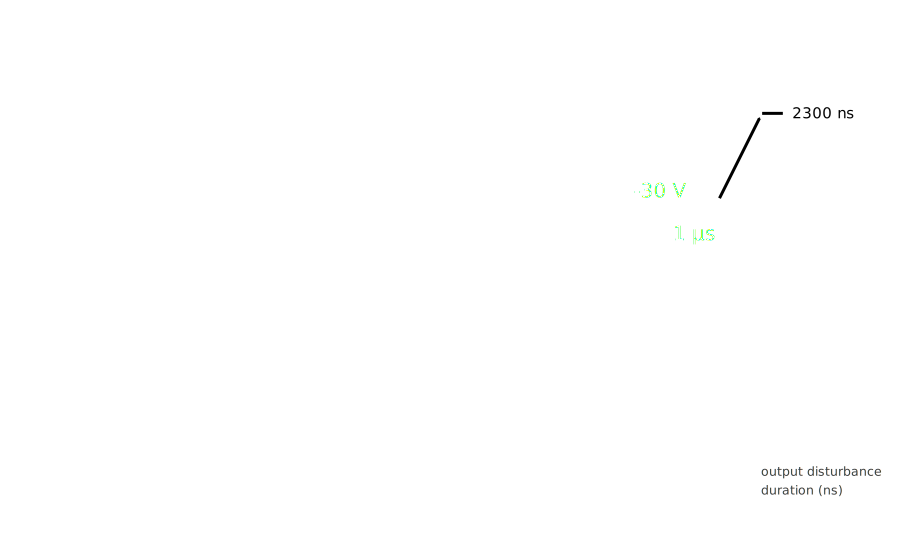
\includegraphics[width=\textwidth]{src/4/figures/preregulator_cz.png}
  \caption{Pre-regulator 9V clamped-output characterization}
  \label{pre_regu_wb}
\end{figure}

\begin{figure}[!htbp]
  \centering
  \includegraphics[width=\textwidth]{src/4/figures/bandgap_cz.png}
  \caption{Bandgap 1.0V reference characterization}
  \label{bandgap_wb}
\end{figure}

\begin{figure}[!htbp]
  \centering
  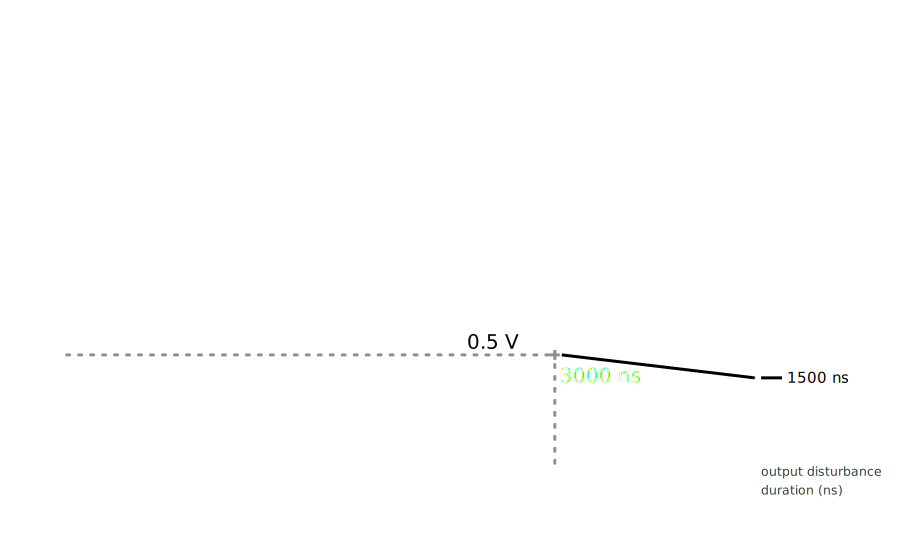
\includegraphics[width=\textwidth]{src/4/figures/regulator_cz.png}
  \caption{Regulator 2.5V supply characterization}
  \label{regu_wb}
\end{figure}

% Characterization done, now perform chaining
After the characterization phase, it is now possible to chain the models together.
The goal is to evaluate the entire function's robustness with the method described in \label{sec:block-chaining}.
A rectangular pulse is injected on the global input (pre-regulator input).
The chain of models is used to predict, without running any more simulations, the failure or not on the output pin.
For the purpose of this test, the input stress will be generated by a \gls{tlp} generator, producing a pulse of 100ns duration and -30V amplitude.

% Do it on one pulse config
%TODO: Review values
First, the coordinaates (100ns, -30V) are reported on curve \ref{pre_regu_wb}, the first block model of the system.
This point indicates a failure on the output of the pre-regulator, for a duration of 500ns.
The failure criteria is 0V on the output.
This gives the next point coordinates (500 ns, 0V).
This point is reported on the bandgap's model, the next block in the system.
Using these coordinates in the curve \ref{bandgap_wb} indicates a failure on the bandgap output for about 800ns.
Since the failure criteria for the bandgap is 0V on the output, the next point coordinates are (800ns, 0V).
They are used as an input on the final block's model (fig. \ref{regu_wb}).
Reporting those coordinates, no failure is expected on the regulator output.

In conclusion, the model chain estimated that for a -30V 100ns stress on the input, the regulation function will not be at fault (output < 2.1V).

% Same analysis but with a TLP stress that will cause a fail
The same analysis is done for a -30V stress but with a longer width of 1us.
The failure on the pre-regulator is then estimated to last 2300 ns.
In turn, the bandgap is estimated to fail during 3000 ns.
Finally, the output of the regulator and thus the entire function is estimated to fail during 1500ns.

% Perform standard complete simulation for reference
Those results are then tested against a complete simulation of the entire regulation function (all three block).
The simulation circuit is given Fig. \ref{fig:reference_simu_circuit}.
This simulation uses transistor-level block models.
It will serve as a reference to compare the model-chain against it.

% How will the simulation be conducted
For this simulation, the same input stress are used than previously, and the global output is monitored for failures.
To check the validity of the models at each stage, intermediate voltages are also monitored, at the output of the pre-regulator and the bandgap.
The simulation of the input, pre-regulator output, bandgap output and final (regulator) output are given fig. \ref{fig:reference_simu}.

\begin{figure}[!htbp]
  \centering
  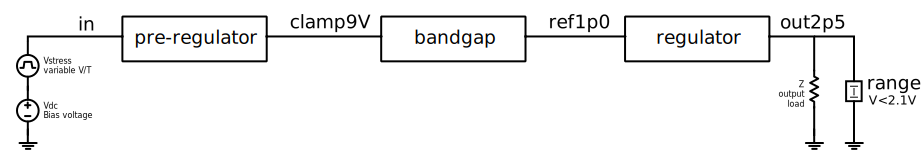
\includegraphics[width=\textwidth]{src/4/figures/complete_simulation_setup.pdf}
  \caption{Complete reference simulation circuit}
  \label{fig:reference_simu_circuit}
\end{figure}

%TODO: Zoom on the area of interest
\begin{figure}[!htbp]
  \centering
  \includegraphics[width=\textwidth]{src/4/figures/total_simulation.png}
  \caption{Reference simulation waveforms}
  \label{fig:reference_simu}
\end{figure}

% Result of the simulation
The simulation showed that for the given stress, the output V(out2p5) will go below 2.1V for 8160ns.
%TODO: Make the comparison with chain models
There is a rather large difference with the model chain.
To try to explain this difference, intermediates nodes are monitored.

% Error at the first block
The output of the pre-regulator is below X V (failure criteria) for XX ns in the full simulation while the model predicted XX ns.
Already, at this first block, there is a large difference between the simulation and the model.

% Error at the second block
The output of the bandgap (second block) shows even a higher difference.
In simulation, the output goes below XX V for XXX ns, while the model predicted XXX ns.

% Conclusion regarding this first simulation
Not only each curve introduces an important error, but errors tend to accumulate after each block.

% Test further simulation vs model
To test further the model versus the reference simulation, a set of different stresses are injected, with different properties.
The goal is to test the model on a larger set of input stresses.
For each stress, the result predicted by the model and the result obtained by the reference simulation are compared.
Results are summarized in table \ref{tab:comparison-multiple-pulses}.
The entire process is summarized in fig. X.

\begin{table}[!htbp]
\centering
\begin{tabular}{@{}|c|c|c|c|@{}}
\toprule
\multicolumn{2}{|c|}{\begin{tabular}[c]{@{}c@{}}Stress\\ properties\end{tabular}} & \multicolumn{2}{c|}{Results} \\ \midrule
duration (ns)                           & amplitude (V)                           & Reference      & Model       \\ \midrule
1 ns                                    & -5V                                     & no fail        & no fail     \\ \midrule
1 ns                                    & -10V                                    &                &             \\ \midrule
1 ns                                    & -15V                                    &                &             \\ \midrule
10 ns                                   & -5V                                     & fail 10ns      &             \\ \midrule
10 ns                                   & -10V                                    &                &             \\ \midrule
10 ns                                   & -15V                                    &                &             \\ \midrule
50 ns                                   & -5V                                     &                &             \\ \midrule
50 ns                                   & -10V                                    &                &             \\ \midrule
50 ns                                   & -15V                                    &                &             \\ \midrule
500 ns                                  & -5V                                     &                &             \\ \midrule
500 ns                                  & -10V                                    &                &             \\ \midrule
500 ns                                  & -15V                                    &                &             \\ \bottomrule
\end{tabular}
\caption{Comparison between simulation and reference for several pulse configurations}
\label{tab:comparison-multiple-pulses}
\end{table}

% Conclusion regarding the tables, differences observed

%TODO Review next
% Where does error come from ? Load impedance
Previously, it was indicated that all WnB curves were extracted with a fixed Zout = 1M\textOmega.
When connected together, each block (pre-regulator, bandgap, regulator) sees a load impedance on its output much different than that.
Thus, it is important to evaluate the impact of this value on the Wunsch and Bell characterization curve.
The pre-regulator is characterized again, this time with a load impedance of 100\textOmega.
This value is rather small impedance, but sufficiently high to not draw too much current on the pre-regulator.
This second characterization is given fig. X.

%TODO: CHARACTERIZATION WITH Z LOW IMPEDANCE

This characterization is compared with the one extracted with 1M\textOmega\.
To make the comparison easier, curves for failure above 1ns, 10ns, 100 ns and 1us were plotted separately (see fig. X).
MAKE COMPARISON

%TODO: COMPARISON Z LOW IMPEDANCE Z HIGH IMPEDANCE 2 * 2 1n -> 1u

SO FAR, CONSIDERED IMPEDANCE AS STATIC AND REAL.
TALK ABOUT IMAGINARY IMPEDANCES, AND DYNAMIC IMPEDANCES

TALK ABOUT ERROR CAUSED BY GRADIENT ?

\subsection{Current limitations}

% Short intro
The bottom-up characterization method helps create higher-order models of circuit functions.
However, preliminary tests regarding this method are inconclusive.
Multiple sources of errors in the modeling method can be found to explain the differences observed.

\subsubsection{Impact of characterization output load}

% First source of error - load impedance
Previously, it was indicated that all characterization curves were extracted with a fixed output load.
In \ref{sec:application-test-vehicle}, the output load Zout was 1M\textOmega.
It is believed that this is the first major source of error.

% Compare 1Mohm with real case where blocks are connected together
In reality, each block (pre-regulator, bandgap, regulator) sees a load impedance on its output much different than 1M\textOmega.
For instance, the output of the pre-regulator is a supply.
As such, it can deliver about 20mA of current while maintaining 8V.
Thus, the minimum output load this block can sustain is 400\textOmega.
The bandgap, on the other hand, provides a reference voltage at 1V but does not deliver a lot of DC current.
More than 1uA is enough to make the output fall of a hundred millivolts.
In this case, the bandgap must see an output impedance of at least 1M\textOmega.

% What is done next
To evaluate the impact the pre-regulator is characterized again, this time with lower load values.
Variations on the input stresses and results are summarized in table \ref{tab:impact-load-on-cz}.

% Analyse the table - worst case
For the smallest 10V stress amplitude, the failure time is largely impacted by the output load.
This is especially true for long pulses.
The worst case is for the -10V 1us pulse.
The output goes below 0V for 1330 ns with 500\textOmega\ on the output, but with 1M\textOmega\, no failure is observed.

% Analyse the table - other cases
However, it is interesting to notice that for larger pulse amplitudes, the output load has a limited impact on the failure duration.
It seems that once the output is at fault, having 500\textOmega\ or 1M\textOmega\ connected to it doesn't change how long it remains at fault.
Fig. \ref{fig:impact-time-domain-load} provides a visual representation of the phenomenon, to try to explain why this result is obtained.
%TODO: Explain more

\begin{figure}[!htbp]
  \centering
  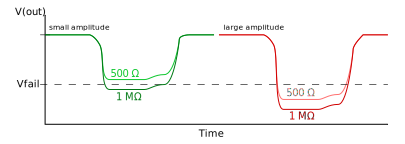
\includegraphics{src/4/figures/zout_impact_time_domain.pdf}
  \caption{Represented impact of output load impedance on the output waveform during a disturbance with a small amplitude (green) and a large amplitude (red)}
  \label{fig:impact-time-domain-load}
\end{figure}

\begin{table}[!htbp]
\centering
\begin{tabular}{llll}
\toprule
load (\textOmega) & amplitude (V) & length (ns) & output disturbed (ns)   \\ \midrule
500               & -10        & 10         & 10n    \\
5k                &            &            & 1n    \\
50k               &            &            & None    \\
1M                &            &            & None    \\
\rowcolor[gray]{.95}
500               &            & 100        & 100n    \\ \rowcolor[gray]{.95}
5k                &            &            & 1n    \\ \rowcolor[gray]{.95}
50k               &            &            & None    \\ \rowcolor[gray]{.95}
1M                &            &            & None    \\

500               &            & 1000       & 1330n    \\
5k                &            &            & 1289n    \\
50k               &            &            & None    \\
1M                &            &            & None     \\
\rowcolor[gray]{.95}
500               & -30        & 10         & 20n    \\ \rowcolor[gray]{.95}
5k                &            &            & 10n    \\ \rowcolor[gray]{.95}
50k               &            &            & 10n    \\ \rowcolor[gray]{.95}
1M                &            &            & 10n    \\

500               &            & 100        &  506n   \\
5k                &            &            &  580n   \\
50k               &            &            &  594n   \\
1M                &            &            &  594n   \\
\rowcolor[gray]{.95}
500               &            & 1000       & 2087    \\ \rowcolor[gray]{.95}
5k                &            &            & 2194    \\ \rowcolor[gray]{.95}
50k               &            &            & 2206    \\ \rowcolor[gray]{.95}
1M                &            &            & 2206    \\

500               & -45        & 10         & 46n    \\
5k                &            &            & 10n    \\
50k               &            &            & 10n    \\
1M                &            &            & 10n    \\
\rowcolor[gray]{.95}
500               &            & 100        & 657n    \\ \rowcolor[gray]{.95}
5k                &            &            & 715n    \\ \rowcolor[gray]{.95}
50k               &            &            & 717n    \\ \rowcolor[gray]{.95}
1M                &            &            & 727n    \\

500               &            & 1000       & 2668n    \\
5k                &            &            & 2764n   \\
50k               &            &            & 2800n    \\
1M                &            &            & 2800n    \\

\bottomrule
\end{tabular}
\caption{Impact of the output load on characterization results}
\label{tab:impact-load-on-cz}
\end{table}

% Talk about static impedances vs dynamic

% Talk about real vs imaginary impedances

\subsubsection{Impact of single level failure criteria}

% Second source of error - single level failure criteria
The use of a single failure criteria per block can introduce an important error as well.
It oversimplifies the response of the output against an input stress.

\subsubsection{Other sources}

%TODO: Make section ? Speak about limitations with multiples nets that are responsible for error propagation
%TODO: Limitation with multiple nets. Interactions between inputs.


On paper, this method was rather promising in terms of applicability.
A block could be characterized once, and reused in different places.
The robustness of a full system could have been quickly and easily deduced from the models of its parts.

However, with the study case exposed earlier, several issues arose that clearly limit the ability of the model to perform as expected.

The main issue with this modelling method is the fact that it relies too much
on the value of the output load for performing the characterization of a block.
This load depends on many different parameters.
And this value will change in function out the block connected on the output (think about block-reuse)
Also, this value may not be constant in frequency.
And this value may also not be constant in time (multiple operating modes, biasing points, etc).

% SHOW SIMULATIONS FOR THIS PROBLEM OF IMPEDANCE VARIATION

% DIRECTIVITY - WE ASSUME STRESS AND FAILURES PROPAGATE FROM INPUT TO OUTPUT. MAY NOT BE THE CASE. ALSO, MAY NOT WORK IN REVERSE WITH SINGLE2MANY BLOCK CONNECTIONS

Another issue, this method is limited to a binary FAIL/NO FAIL criteria.
Not only this criteria is arbitrary (in some cases, the specification could be used to set it), but
for most purely-analog blocks, there will not be a clear failure, rather, most
nets will have degraded values until maybe biasing of the block completely fails.
In this case, the binary criteria hides a lot of information about the degradation.

ANY CLUES TO OVERCOME THESE ISSUES ?

ALSO, FAILURE MAY NOT PROPAGATE IN THIS ONLY WAY, BUT BACKWARD TOO

The main reason why this approach was investigated was for its very interesting modularity
that was highly suitable for block reuse workflow.

However, because of the intrisic interactions between block functions in an integrated circuit,
TRY TO EXPRESS BETTER WHAT PRINCIPLE OF THIS METHOD BOUNDS IT TO FAIL

this approach seems to be bound to fail for building a reusable model for an IC block that could predict
ESD failures at the architecture level and during the IC architecture phase.

\subsection{Proposed workaround}

%
In the current approach, blocks are characterized using a fixed failure criteria on the output.
It results in a characterization table, describing the duration of the output disturbance from the width and amplitude of the input stimulus.
To remove and replace the failure criteria, the same exact approach is proposed.
Since the output duration is calculated with a table, then the output amplitude could be calculated using another table as well.

% New model description
The new model contains two 2D tables instead of one, and the new table associates an output amplitude to an input width and amplitude.
Fig. \ref{fig:principle-transfert-func-v2} summarizes the new model.
\textbf{Table A} is the amplitude table, to calculate the \textbf{amplitude} of the output disturbance.
\textbf{Table W} is the width table, to calculate the \textbf{duration} of the output disturbance.

\begin{figure}[!h]
  \centering
  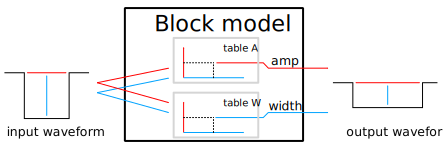
\includegraphics{src/4/figures/principle_transfert_function_v2.pdf}
  \caption{Improved modeling method}
  \label{fig:principle-transfert-func-v2}
\end{figure}

% What changes in the characterization
To extract both tables, the process is a bit different from the first methodology.
For each characterization simulation, the maximum output amplitude is recorded.
It is stored in table A.
The duration is measured on the output at 90\% of this maximum amplitude.
The validity of this threshold is discussed after in \ref{sec:limits-block-cz-final}.

% What does not change
The rest of the methodology remains identical.
In particular, model chaining is performed the same way since block models still accept and input width/disturbance and return an output width/disturbance.

% Summary of the process
%Fig. \ref{fig:full-method-v2} summarizes the entire characterization and chaining process for a 2-block setup.
%Each block is characterized, generating the two tables mentionned earlier.
%Then, using both tables, an input stress of 50V 100ns becomes a 12V 350ns disturbance after the first block, and a 3V 4000 ns after the second block.

%\begin{figure}[!h]
%  \centering
%  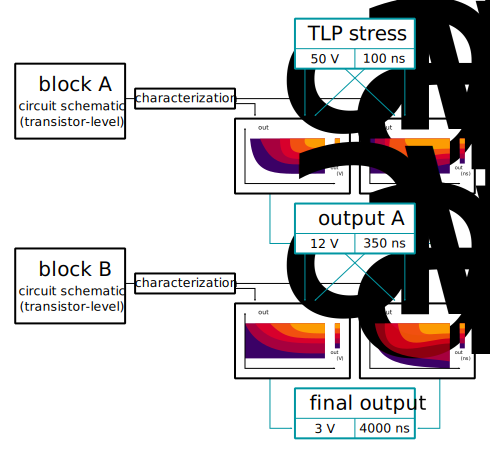
\includegraphics[width=0.7\textwidth]{src/4/figures/full_method_overview_v2.pdf}
%  \caption{Overview of improved bottom-up method - example with two blocks}
%  \label{fig:full-method-v2}
%\end{figure}

\subsubsection{Application of the improved method}

The new characterization method is applied to all three blocks of the regulation function.
The amplitude table of the pre-regulator is plotted in Fig. \ref{fig:pre_regu_amp} and the width table in Fig. \ref{fig:pre_regu_width}.
Different patterns can be observed between both figures.
The output amplitude gradient seems independent from the input width because it displays only horizontal lines, and depends only on the input amplitude.
The output duration gradient is a lot more complex with multiple different patterns.
Overall, large input amplitude and duration tend to result in long output disturbances.
The other characterization tables of the bandgap and pre-regulator are provided in Annex \ref{apx:block-cz}.

\begin{figure}[!h]
  \centering
  \includegraphics[width=\textwidth]{src/4/figures/vpre_cz_v2_amplitude.png}
  \caption{Pre-regulator V\textsubscript{clamp9} amplitude matrix}
  \label{fig:pre_regu_amp}
\end{figure}

\begin{figure}[!h]
  \centering
  \includegraphics[width=\textwidth]{src/4/figures/vpre_cz_v2_width.png}
  \caption{Pre-regulator V\textsubscript{clamp9} width matrix}
  \label{fig:pre_regu_width}
\end{figure}


% What is done for validation
The chaining process is performed again with a -30V 1 \textmu{}s rectangular input stimulus.
The reference curve and reference test setups remain identical to the ones presented earlier (Fig. \ref{fig:reference_simu_circuit}).

% Result of the chaining process
The chaining process predicts that V\textsubscript{clamp9} will be down at -1.6V during 1800 ns.
The 1.6V value is obtained by taking coordinates of the input stimulus (-30V, 1 \textmu{}s) and applying them to Fig. \ref{fig:pre_regu_amp}.
1.6V then corresponds to the gradient value at those coordinates.
The 1800ns is obtained with the same input coordinates but applied to Fig. \ref{fig:pre_regu_width} instead.
The same process is then used for the bandgap and the regulator.
V\textsubscript{1p0} is predicted at -1.25V during 3300 ns.
V\textsubscript{2p5} is predicted at 2.0V during 2700 ns.
Those values are employed for generating model waveforms, and are compared to the reference simulation in Fig. \ref{fig:reference_simu_v2}.

% Curve analysis
The model matches correctly the simulation of V\textsubscript{clamp9}, both in terms of amplitude and width.
The width is slightly underestimated but overall the result is acceptable.
For V\textsubscript{1p0}, the width is extremely well reproduced, but the amplitude is about twice the reference value.
It seems that taking the minimum amplitude value during the characterization is not ideal.
This error should be investigated further to determine the actual root cause and provide a solution.
The last signal V\textsubscript{2p5} shows a quite good correlation despite the fact that it is a triangle-like waveform.
More validations were performed with (-20V, 1\textmu{}s) and (-20V, 100ns) stimuli.
The results are provided in appendix \ref{apx:block-model-comparison}.
Overall, the modifications brought to the modeling method seemed to have a positive impact on the curve models.
A lot of room is left for improvements, in particular for reproducing the bandgap output signal V\textsubscript{1p0} that systematically suffers from amplitude modeling error.

\begin{figure}[!h]
  \centering
  \includegraphics[width=\textwidth]{src/4/figures/total_simulation_30V_1u_V2.png}
  \caption{Reference simulation waveform : TLP stress -30V 1\textmugreek{}s }
  \label{fig:reference_simu_v2}
\end{figure}

% Conclusion, it works for this case
This section presented a potential improvement over the model chain method initially proposed.
This technique showed good results and seems promising for quickly estimating the robustness of a high-level integrated function.
The next section discusses further improvements for extracting width and amplitude during characterization.

\subsubsection{Potential improvements regarding parameters extraction}

% What is the challenge regarding the extraction of the models
In the simulations described earlier, a single width and maximum amplitude per waveform were extracted manually.
However, waveforms are never perfectly squared, and an width and amplitude cannot always be extracted easily.
The challenge is to find the right rule for simplifying them into a rectangular waveform, and extracting the two parameters.
This applies to the input waveform and the output waveform during the characterization of a block.

% First approach with a 90% amplitude
Initially, the rules were to set $V$ equal to the maximum value of the waveform (input or output), and $W$ the width of the pulse at 90\% of $V$.
This waveform simplification into a rectangular shape can be difficult to perform with some non-trivial curves.
Two cases where this simplification is not straightforward are illustrated in Fig. \ref{fig:impact-single-failure-criteria}.

\begin{figure}[!h]
  \centering
  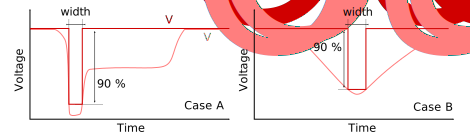
\includegraphics[width=\textwidth]{src/4/figures/better_output_modelling.pdf}
  \caption{Improved output modeling method based on 90\% of maximum disturbance amplitude}
  \label{fig:impact-single-failure-criteria}
\end{figure}

% Explain case A
Case \textit{A} is often observed during the injection of an electrostatic discharge.
The \gls{esd} signal is superimposed on top of a slow signal variation.
In that case, the waveform exhibits a very short, high amplitude peak, followed by slower smaller-amplitude variation.
The width of the pulse is much shorter than the original curve, leading the model to be very inaccurate.

% Explain case C
Case \textit{B} is observed on nets with high capacitive coupling to ground.
Those signals are not directly disturbed by the \gls{esd}, but the block that drives them can go into reset.
In this situation, the nets slowly decreases then, once functionality resumes, the nets goes back to its nominal value.
With the 90\% threshold, a large area of the disturbed waveform is missing in the model, making it very inaccurate.

% What is the consequence
In both those cases, the 90\% threshold leads to underestimating the total disturbance width.
The modeled waveform has a much smaller duration and area than the original one.
Overall, it was observed that the model and original waveform areas should be close for the models to work.

% The relative threshold is not good enough, a smarter technique is required
Instead of focusing on the peak amplitude, a smarter method is required.
Ideally, it needs to extract a width and amplitude that would result in the same area than the original waveform, while looking as similar as possible.

A feature detection method using amplitude distribution could be performed to identify key amplitudes in the waveforms.
Other techniques could be conceived, such as conbining multiple rectangular waveforms to describe more complex waveforms.
Basically, it would consist in breaking down a complex waveform into 2 or more rectangles, and applying each rectangle to the model chain.
This waveform breakdown concept is illustrated in Fig. \ref{fig:waveform-deconvolution}.

\begin{figure}[!h]
  \centering
  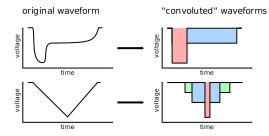
\includegraphics[width=0.7\textwidth]{src/4/figures/shape_convolution.pdf}
  \caption{Waveform breakdown into rectangular shapes}
  \label{fig:waveform-deconvolution}
\end{figure}

\subsection{Final conclusion and follow-up work}
\label{sec:limits-block-cz-final}

% Sum up what was done
In this section, principles were detailed for a block modeling method, targeting powered integrated functions exposed to disturbances.
It initially started off from the Wunsch and Bell method \cite{wunsch-bell}, which is based on a pass/fail failure criteria and targets hard-failure of electronic devices.
The method was improved to fit better the modeling of analog functions, symbolized by an input, and output and a transfer function.
The failure criteria was then removed because it was a large source of error.
The final model is constituted of two characterization tables.
The first one describes the \textbf{output amplitude} as a function of the input amplitude and duration.
The second one describes the \textbf{output duration} as a function of the input amplitude and duration.
For this purpose, waveforms observed on the inputs and outputs were simplified as rectangular shapes.
Each table stores the transient response of the characterized block against a wide range of input disturbance configurations.
On a single study-case, it was shown that this method is able to reproduce simplified waveforms of a disturbance propagating through a chain of block functions.

% Limitations
Some limitations must be overcome before this method can be applied to a larger scale.
So far, only very linear circuit topologies were considered.
A single input net and output net was studied per block.
It is one-to-one relation.
In reality, the relations are closer to many-to-one or many-to-many.
A single input will impact multiple outputs when disturbed.
Inputs do not have isolated impact, multiple inputs will affect the same group of outputs when they get stressed.

Also, more study cases are required to verify further the hypothesis under which ESD simulations at silicon-level can be performed using exclusively rectangular pulses, to disturb blocks in isolated testbenches.


\section{Top-down modeling approach}

Unlike the bottom-up modeling approach, the top-down considers an IC in terms of
externally-exposed IO, and a specification regarding the state of these IOs.

The main advantage compared to the bottom-up method, is that where there was no
way to set a clear failure criteria with the bottom-up, using the top-down, the
product specification serves as a clear reference for defining failures.

Indeed, we can consider using this specification to say that, during an ESD,
any signal that goes outside its nominal range is at fault.

Then, the idea is to inject the ESD on an input pin, and observe if some output
pins go out of specification, and so, in fault.

Another advantage of this method is the abstraction over the design. Since it is
easy to probe pins of the IC, we can measure voltage/current at those pins fairly
easily, and derive models from those values, without needing the access the chip's internals.

The question is, is this sufficient to build an accurate enough model ?

\subsection{Characterization}
Apply variable width/variable height stress

Talk about injection setup. Move away from DPI system

\subsection{Failure modeling}
Make failure model + IO model
Use it in other simulations (Gun for instance), to check if failure level can be predicted

\section{Functionnal block checks}

In this section, another bottom-up method is proposed.
Like detailed previously, bottom-up methods are interesting for the intrisic modularity and reusability they offer.

In section 4.2, a block-failure modeling approach was detailed.
Mainly, it focused on modeling the failure of a block as a time and amplitude criteria on an input.
By going beyond the criteria, a failure was generated, and the output was put at fault.
This fault was propagated then further in the system.
The main issue with this approach is the strong coupling between blocks.
To check that an input did not violate its failure criteria, you needed to know information about its surrounding blocks.

In this section, the method is also bottom-up but we focus instead on the signals inside the block itself, and not at its boundaries.
The idea is to write a set of rules or assertions on a few signals inside the block.
When those rules are violated, we know the block is in a faulty state.

This approach offers two main advantages compared to the section 4.2 method.

First, the rules are written logically based on the design of the block, and not arbitrariraly defined.
If for instance a net is the gate command of a current mirror, a few criteria can be derived logically.
For the current mirror to function properly, at least 1 gate voltage is required for biasing.
Going below this voltage, the current mirror will not perform its copy anymore.

SCHEMATIC SIMPLE CURRENT MIRROR

Another example is taking a regulator.
If current drawn on the output of the regulator exceeds nominal capability, then the block will be considered faulty.

A set of simple rules could also be derived on supplies and ground.
For all blocks, supplies should be expected within a given range.
Grounds should be expected close to 0, and most likely lower than a body diode triggering voltage.

The second major advantage is that the rules are specific to a block.
They do not depend on boundary blocks, because they focus on the logical behavior of the block itself.
This means that this approach is highly modular and scalable.
Indeed, a set of rules written with an IP can travel with the block.
In any project/IC the block will be used, the rules will apply.

\subsection{Problem solved}
Why are assertions useful ?
Inherent scale factor and complexity makes inspecting the top-cell and all its sub cells impossible for a human.
Need an automated checking system, that runs for any simulation (ESD or other).

\subsection{Applicability}

Determine automatically in a top simulation (or simplified top) which blocks/nets went out of spec and so at fault.
Also, determine mistakes when building testbenches.
Also, constitute an electrical documentation of the block block.
Also, determine during DC spec if all blocks are properly started.
Also, determine connection issues (floating ground and nets).

Potential integration in Cadence environment
So far, limited support for assertions in Cadence.
In an ideal case, assertion files should be a specific view of the asserted cell.
This way, when the cell is copied or moved around, the assertions will move with it and be reused.

\subsection{Perks and Drawbacks}

Simple to write.
Reusable.
Integrates well into the design flow
General purpose (not limited to ESD, very useful in general considering all applications).

DRAWBACKS ?

\subsection{Proof of concept with a simple study-case}

EVEREST ?
SIMPLE CIRCUIT IN SIMULATION ?

\subsection{Proposed debugging interface}

User interface proposal for monitoring assertions.
Visualize when circuit is ready (all assertions are gree)
During and after ESD, which nets/blocks are disturbed first, how disturbances propagate inside the circuit.

\section{Application of Wunsch & Bell curves to arbitrary waveforms}
\label{sec:wb-for-arbitrary-wvfs}

% WB here based on amplitude/duration of square pulse
WB

% Reality is more arbitratry, time varying pulse

\subsection{Integration method}

% Explain what this method is
Integration

\subsection{Amplitude-distribution method}

% Explain what this method is
Distribution


% End of chapter files listing

% Conclusion
\chapter{Conclusion}
\label{sec:final-conclusion}

To be done.


% Appendix
\bookmarksetupnext{level=part}
\begin{appendices}
\chapter{TLP modeling}
\section{Validation curves}
\label{apx:tlp-validation-curves}

\begin{figure}[!h]
  \centering
  \includegraphics[width=\textwidth]{src/2/figures/tlp_comparison_open_10V.png}
  \caption{Voltage and current waveforms comparison : \SI{10}{\volt} charging voltage on open circuit}
  \label{fig:comparison-tlp-open-10v}
\end{figure}

\begin{figure}[!h]
  \centering
  \includegraphics[width=\textwidth]{src/2/figures/tlp_comparison_open_1000V.png}
  \caption{Voltage and current waveforms comparison : \SI{1000}{\volt} charging voltage on open circuit}
  \label{fig:comparison-tlp-open-1000V}
\end{figure}

\begin{figure}[!h]
  \centering
  \includegraphics[width=\textwidth]{src/2/figures/tlp_comparison_short_10V.png}
  \caption{Voltage and current waveforms comparison : \SI{10}{\volt} charging voltage on a short circuit}
  \label{fig:comparison-tlp-short-10V}
\end{figure}

\begin{figure}[!h]
  \centering
  \includegraphics[width=\textwidth]{src/2/figures/tlp_comparison_short_1000V.png}
  \caption{Voltage and current waveforms comparison : \SI{1000}{\volt} charging voltage on a short circuit}
  \label{fig:comparison-tlp-short-1000V}
\end{figure}

\begin{figure}[!h]
  \centering
  \includegraphics[width=\textwidth]{src/2/figures/tlp_comparison_R25_10V.png}
  \caption{Voltage and current waveforms comparison : \SI{10}{\volt} charging voltage on \SI{25}{\ohm}}
  \label{fig:comparison-tlp-load-10v}
\end{figure}

\begin{figure}[!h]
  \centering
  \includegraphics[width=\textwidth]{src/2/figures/tlp_comparison_R25_1000V.png}
  \caption{Voltage and current waveforms comparison : \SI{1000}{\volt} charging voltage on \SI{25}{\ohm}}
  \label{fig:comparison-tlp-load-1000v}
\end{figure}

\begin{figure}[!h]
  \centering
  \includegraphics[width=\textwidth]{src/2/figures/tlp_comparison_470nH_500V.png}
  \caption{Voltage and current waveforms comparison : \SI{500}{\volt}charging voltage on a \SI{470}{\nano\henry} inductor}
  \label{fig:comparison-tlp-inductor}
\end{figure}

\chapter{Block characterizations}
\section{Characterizations}
\label{apx:block-cz}

\begin{figure}[!h]
  \centering
  \includegraphics[width=\textwidth]{src/4/figures/bandgap_cz_v2_amplitude.png}
  \caption{Bandgap V\textsubscript{clamp9} amplitude matrix}
  \label{fig:bg_amp}
\end{figure}

\begin{figure}[!h]
  \centering
  \includegraphics[width=\textwidth]{src/4/figures/bandgap_cz_v2_width.png}
  \caption{Bandgap V\textsubscript{clamp9} width matrix}
  \label{fig:bg_width}
\end{figure}

\begin{figure}[!h]
  \centering
  \includegraphics[width=\textwidth]{src/4/figures/regulator_cz_v2_amplitude.png}
  \caption{Regulator V\textsubscript{clamp9} amplitude matrix}
  \label{fig:regu_amp}
\end{figure}

\begin{figure}[!h]
  \centering
  \includegraphics[width=\textwidth]{src/4/figures/regulator_cz_v2_width.png}
  \caption{Regulator V\textsubscript{clamp9} width matrix}
  \label{fig:regu_width}
\end{figure}

\chapter{Black box modelling}
\section{Additional validations}
\label{apx:black-box-validations}

\begin{figure}[!h]
  \centering
  \includegraphics[width=\textwidth]{src/4/figures/comparison_model_total_20V.png}
  \caption{Comparison of complete schematic and model simulations for input port (\SI{20}{\volt} TLP)}
  \label{fig:compare-model-simu-20}
\end{figure}

\begin{figure}[!h]
  \centering
  \includegraphics[width=\textwidth]{src/4/figures/comparison_model_total_40V.png}
  \caption{Comparison of complete schematic and model simulations for input port (\SI{40}{volt} TLP)}
  \label{fig:compare-model-simu-40}
\end{figure}

\end{appendices}


% Bibliography
\bibliographystyle{unsrt}
\cleardoublepage
\phantomsection
\addcontentsline{toc}{chapter}{Bibliography}
\bibliography{../src/refs}
\printindex

% List of code snippets
%\listoflistings

% Glossary
\setglossarystyle{altlist}
\printglossaries

\end{document}
